\documentclass{article}
\usepackage{hyperref}
\usepackage{graphicx}
\usepackage{float}
\usepackage{a4wide}
\usepackage[utf8]{inputenc}
\usepackage[portuguese]{babel}

\hypersetup{
    colorlinks=true,
    linkcolor=black,
    filecolor=magenta,      
    urlcolor=cyan,
}

\setlength{\parindent}{0pt}

\begin{document}
\begin{titlepage}
    % Logo e instituição
    \begin{flushleft}
        
\includegraphics[width=0.2\textwidth]{logo.png}
    \end{flushleft}    
    \begin{flushleft}
        \textbf{Departamento de Informática} \\
        \textbf{Escola de Engenharia} \\
        \textbf{Universidade do Minho}
    \end{flushleft}    
    \vspace{2cm}

    % Título do trabalho
    \begin{center}
        {\Huge \textbf{Gestor de Turnos}} \\
        \vspace{0.5cm}
    \end{center}
    
    % Curso e ano
    \begin{center}
        \textbf{Interface Pessoa-Máquina} \\
        Licenciatura em Engenharia Informática \\
        2024/2025
    \end{center}

    \begin{center}
    \href{https://www.figma.com/design/8PO30QoW6AGILm8vvlVg2B/SWAP2?t=lgVA4g5Cron9eMVb-1}{Link para o projeto}
    \end{center}

    \begin{figure}[H]
        \centering
        
\includegraphics[width=0.25\linewidth]{carolina.png}
        
\includegraphics[width=0.25\linewidth]{diogo.png}
        
\includegraphics[width=0.25\linewidth]{esteves.jpg}
        \label{fig:enter-label}
    \end{figure}
    \begin{figure}[H]
        \centering
        
\includegraphics[width=0.25\linewidth]{ze.png}
        
\includegraphics[width=0.25\linewidth]{rodrigo.jpg}
        \label{fig:enter-label}
    \end{figure}

    \vfill
    % Grupo e autores
    \begin{flushright}
        \textbf{Grupo 01} \\
        Ana Cerqueira, a104188 \\
        Diogo Barros, a100751 \\
        Diogo Esteves, a104004 \\
        José Lopes, a104541 \\
        José Matos, a100612 \\
        \vspace{0.5cm}
        04/05/2025
    \end{flushright}
\end{titlepage}

\tableofcontents

\newpage
\section{Objetivos do Trabalho}
O principal objetivo deste trabalho consistiu no desenvolvimento de uma aplicação web interativa que permita a gestão de turnos académicos por parte dos estudantes e do diretor do curso, com funcionalidades de troca rápida de turnos. A aplicação visa simular um sistema de comunicação assíncrona entre estudantes, facilitando o envio, receção e gestão de pedidos relacionados com os seus horários.\newline
De forma mais concreta, pretendeu-se atingir os seguintes objetivos:

\begin{itemize}
    \item Criar uma interface intuitiva onde o estudante possa consultar os seus turnos atribuídos.
    \item Permitir o envio de mensagens entre o diretor de curso e professores/estudantes.
    \item Gerir o estado de mensagens (enviadas, recebidas, lixo), criando uma caixa de correio digital.
    \item Permitir o diretor do curso de gerir os turnos de cada uma das Unidades Curriculares.
    \item Permitir o diretor de curso consultar e gerir as alocações de cada um dos alunos, bem como consultar o perfil destes.
\end{itemize}
Além disso, foi de especial importância desenvolver um horário modular e responsivo, de forma a apresentar o máximo número de turnos ao mesmo tempo sem sacrificar a interface visual ou a experiência do utilizador.

\newpage
\section{Descrição de Alterações ao Protótipo}
Durante o desenvolvimento da aplicação, algumas alterações ao protótipo inicialmente proposto na Fase 1 foram introduzidas, com o objetivo de melhorar a experiência do utilizador e simplificar a lógica de implementação. Estas alterações, justificadas tanto por questões de design como por motivos técnicos, são descritas de seguida:

\begin{itemize}
    \item \textbf{Indicação visual de turnos cheios (\textit{não implementada})}: estava inicialmente previsto que turnos com o número máximo de alunos fossem assinalados com uma cor distinta, acompanhados por um rótulo com o número atual e o número máximo de estudantes (ex: 35/40). No entanto, optou-se por não incluir esta funcionalidade na versão final, uma vez que, na prática, introduzia demasiado ruído visual na interface e dificultava a leitura dos turnos. A decisão foi tomada para preservar a clareza da interface.

    \item \textbf{Remoção da notificação após envio de mensagem}: no protótipo original, estava prevista uma notificação visual a confirmar o envio de mensagens. Esta funcionalidade foi retirada, passando o envio de mensagens a ocorrer de forma direta e silenciosa, com impacto imediato na caixa de correio. Esta decisão simplificou a experiência do utilizador e eliminou passos desnecessários, tornando o processo mais fluido.

    \item \textbf{Ícones de navegação sempre visíveis}: em vez de esconder os ícones de navegação baseado na página atual do utilizador, decidiu-se mantê-los sempre visíveis, mas com um aspeto atenuado (uma cor mais escura). Esta abordagem melhora a consistência da interface e ajuda o utilizador a perceber melhor o estado atual da aplicação, bem como os efeitos quando navega entre páginas.

    \item \textbf{Remoção do filtro por turno}: o filtro que permitia ao utilizador restringir a lista de turnos por turno foi removido. Esta decisão prendeu-se com a perceção de que o filtro, embora funcional, complicava a interface sem trazer valor significativo na maioria dos casos.
\end{itemize}
Estas alterações refletem uma abordagem centrada no utilizador, onde a clareza da interface e a simplicidade das interações foram priorizadas. Optou-se por sacrificar certas funcionalidades planeadas que, embora tecnicamente viáveis, não contribuíam positivamente para a experiência final.

\newpage
\section{Descrição da Implementação}
A solução para a aplicação desenvolvida foi implementada com recurso ao framework Vue 3, utilizando a Composition API, e faz uso de diversas bibliotecas auxiliares para gestão de estado, comunicação com o backend e organização de componentes.

\subsection{Estrutura e Decomposição em Componentes}
A aplicação está dividida em múltiplas páginas (views), cada uma representando funcionalidades específicas. Os componentes foram organizados em três níveis principais:

\begin{itemize}
    \item \textbf{Templates}: componentes de layout que organizam a estrutura visual da página (ex: MessagesTemplate.vue).
    \item \textbf{Views}: páginas que lidam com lógica de carregamento e ligação entre dados e os templates (ex: MessagesPage.vue).
    \item \textbf{Stores}: gestão de estado com Pinia, permitindo persistência local e sincronização com o backend (ex: allocationStore.ts, messagesStore.ts, userInboxStore.ts).
\end{itemize}
Além disso, as templates foram montadas a partir de componentes que, por sua vez, poderiam utilizar dentro de si outras componentes a niveis mais elementares. Por exemplo, a página de alunos (StudentPage.vue) monta a template (StudentTemplate.vue). Esta template é de seguida construída a partir de várias outras componentes elementares (como ShiftSelector.vue).

\subsection{Lógica de Negócio}
A lógica de negócio também foi separada por responsabilidades, onde cada uma das \textit{stores} gere uma entidade da base de dados. Por exemplo:

\begin{itemize}
    \item A \texttt{messagesStore} gere o conjunto global de mensagens e permite ações como aprovar, rejeitar, mover para o lixo e restaurar.
    \item A \texttt{userInboxStore} faz a gestão da caixa de entrada, enviados e lixo, por utilizador.
    \item A \texttt{allocationStore} gere as alocações dos estudantes a turnos específicos.
    \item A \texttt{scheduleStore} mantém os eventos e turnos disponíveis.
\end{itemize}
Deste modo, a aplicação segue um padrão reactivo, onde alterações feitas pelos utilizadores atualizam automaticamente o estado local e são depois propagadas para o backend a partir de operações de sincronização.

\subsection{Estrutura da Base de Dados}
A base de dados utilizada é um ficheiro JSON servido por \texttt{json-server}. A estrutura foi desenhada de forma a representar entidades fundamentais como mensagens, utilizadores, eventos e alocações.
As principais entidades presentes são:

\begin{itemize}
    \item \textbf{courses}: cada UC é representada por nome, abreviação, semestre e curso.
    \begin{verbatim}
    {
      "id": 3,
      "courseId": "Laboratórios de Informática I",
      "name": "LI1",
      "semester": 1,
      "degreeId": 1
    }
    \end{verbatim}
    
    \item \textbf{shifts}: cada turno contém o nome, a sua UC, a sala, o professor, o número de alunos alocados e a data e hora.
    \begin{verbatim}
    {
      "id": 2,
      "courseId": 1,
      "classroomId": 1,
      "day": "Ter",
      "from": 10:00",
      "to": "12:00",
      "name": "PL1",
      "teacherId": 92001,
      "totalStudentsRegistered": 15
    }
    \end{verbatim}
    
    \item \textbf{allocations}: representa a alocação de um estudante a um turno.
    \begin{verbatim}
    {
      "id": 1,
      "studentId": 104302,
      "shiftId": 30
    }
    \end{verbatim}
\end{itemize}

\subsection{Bibliotecas e Ferramentas Utilizadas}
\begin{itemize}
    \item \textbf{Vue 3 + Vite}: base da aplicação, permitindo desenvolvimento rápido com hot-reload, modularidade e performance.
    \item \textbf{Pinia}: biblioteca oficial de gestão de estado para Vue. Substitui o Vuex com uma abordagem mais simples e compatível com o Composition API.
    \item \textbf{Vue Router}: para navegação entre páginas, utilizando rotas dinâmicas com parâmetros (/messages/:userId).
    \item \textbf{TypeScript}: tipagem estática, garantindo maior robustez e previsibilidade no código.
    \item \textbf{json-server}: utilizado como mock backend para simular chamadas GET, POST, DELETE, etc., num ambiente RESTful local.
    \item \textbf{ESLint + Prettier}: ferramentas de linting e formatação automática de código, garantindo consistência no estilo de escrita.
\end{itemize}

\subsection{Comunicação com o Backend}
A comunicação com o backend é feita através de chamadas \texttt{fetch} diretas para endpoints REST simulados com \texttt{json-server}. As operações seguem os métodos tradicionais:

\begin{itemize}
    \item \texttt{GET} para leitura de dados (/allocations, /messages, /shifts)
    \item \texttt{POST} para criação de novos registos
    \item \texttt{DELETE} para remoção de alocações antigas
\end{itemize}

O estado local é sincronizado com o servidor manualmente quando necessário, através de funções como \texttt{syncAllocations()} e \texttt{syncChanges()}.

\newpage
\section{Reflexão sobre a Aplicação Desenvolvida na Perspetiva do Utilizador}

A aplicação desenvolvida tem como principal objetivo permitir a gestão de trocas de turnos entre estudantes de forma intuitiva, rápida e eficiente. Tendo em conta a perspetiva do utilizador, foram identificados diversos pontos fortes e algumas limitações, que se discutem de seguida.

\subsection{Pontos Fortes}

\begin{itemize}
    \item \textbf{Interface clara e responsiva}: A utilização do Vue 3 em conjunto com boas práticas de organização de componentes permitiu desenvolver uma interface reativa e responsiva. As transições entre páginas e a atualização dos dados ocorrem de forma fluída, com feedback visual imediato ao utilizador.
    
    \item \textbf{Simplicidade nas ações}: O processo de troca de turnos foi desenhado para ser direto e intuitivo. Os utilizadores conseguem enviar pedidos de troca ou remoção de forma simples, sem passos intermediários confusos.
    
    \item \textbf{Feedback visual consistente}: Os botões e ícones de ação mantêm-se visíveis mesmo quando as ações não estão disponíveis, apresentando-se atenuados (\textit{grayed out}). Esta abordagem melhora a previsibilidade e evita situações de frustração, onde o utilizador não entende por que razão um botão desapareceu.
    
    \item \textbf{Separação clara das mensagens}: A divisão entre mensagens recebidas, enviadas e lixo ajuda o utilizador a localizar rapidamente os pedidos relevantes, reduzindo a complexidade de navegação.
    
    \item \textbf{Estrutura modular e escalável}: A separação em \texttt{stores} e componentes reutilizáveis permite uma manutenção mais fácil da aplicação e futuras extensões com novas funcionalidades.
\end{itemize}

\subsection{Pontos Fracos}

Apesar dos pontos positivos, existem ainda áreas que podem ser melhoradas:

\begin{itemize}
    \item \textbf{Contraste insuficiente de cores}: Um dos problemas mais relevantes identificado prende-se com a acessibilidade. Testes realizados com a ferramenta \texttt{Pa11y} revelaram que a aplicação falha em vários critérios de contraste de cor. Este problema tem origem no protótipo inicial, onde foram escolhidas combinações de cores com baixo contraste (ex: texto claro sobre fundos brancos ou azuis-claro). Este aspeto compromete a legibilidade da interface para utilizadores com dificuldades visuais e não respeita os níveis mínimos exigidos pelo WCAG 2.1.

    \item \textbf{Ausência de confirmações visuais em certas ações}: Embora a remoção de notificações de envio tenha simplificado a experiência, em alguns casos (como quando uma troca é aprovada) pode ser útil apresentar uma confirmação mínima para reforçar ao utilizador que a ação foi completada com sucesso.

    \item \textbf{Falta de mecanismos de filtro e ordenação}: Torna-se evidente a falta de alguns mecanismos de filtro ou ordenação, principalmente no âmbito de procura de estudantes. A aplicação não tem qualquer meio de procura de alunos por nome, semestre inscrito ou até número de aluno.

    \item \textbf{Dependência de sincronizações manuais}: Algumas ações exigem chamadas explícitas ao backend para sincronizar dados (\texttt{syncChanges}, \texttt{syncAllocations}). Embora estas operações funcionem corretamente, um sistema de sincronização automática ou em segundo plano traria maior transparência ao utilizador.
\end{itemize}

\subsection{Testes de Acessibilidade com Pa11y}

Foi utilizado o analisador automático \texttt{Pa11y} para verificar o cumprimento de normas básicas de acessibilidade (WCAG 2.1). Os testes foram realizados sobre as principais páginas da aplicação, nomeadamente:

\begin{itemize}
    \item Página de login
    \item Página de gestão administrativa (diretor do curso)
    \item Página de gestão de alocações
    \item Página do estudante
    \item Página de mensagens (inbox) e de criação de mensagens
\end{itemize}
Os resultados revelaram conformidade geral com os critérios técnicos, sem erros estruturais críticos. No entanto, destacou-se consistentemente o problema do baixo contraste entre cores, já referido anteriormente. Esta falha será documentada no repositório do projeto através dos relatórios exportados.

\subsection{Considerações Finais}

A aplicação consegue cumprir o seu objetivo central de facilitar trocas de turno entre estudantes, com uma experiência de utilização simples, coesa e fluída. As principais oportunidades de melhoria prendem-se com a acessibilidade (contrastes) e algumas pequenas melhorias na experiência de interação. De futuro, seria também pertinente realizar testes de usabilidade com utilizadores reais para validar as decisões tomadas e recolher feedback qualitativo.

\newpage
\section{Manual de Utilização}
De seguida, são apresentadas instruções sobre como utilizar a aplicação, incluindo uma explicação das ações possíveis, os seus efeitos, e uma descrição das páginas e popups disponíveis para os utilizadores.

\subsection{Descrição das Páginas}
\begin{figure}[H]
    \centering
    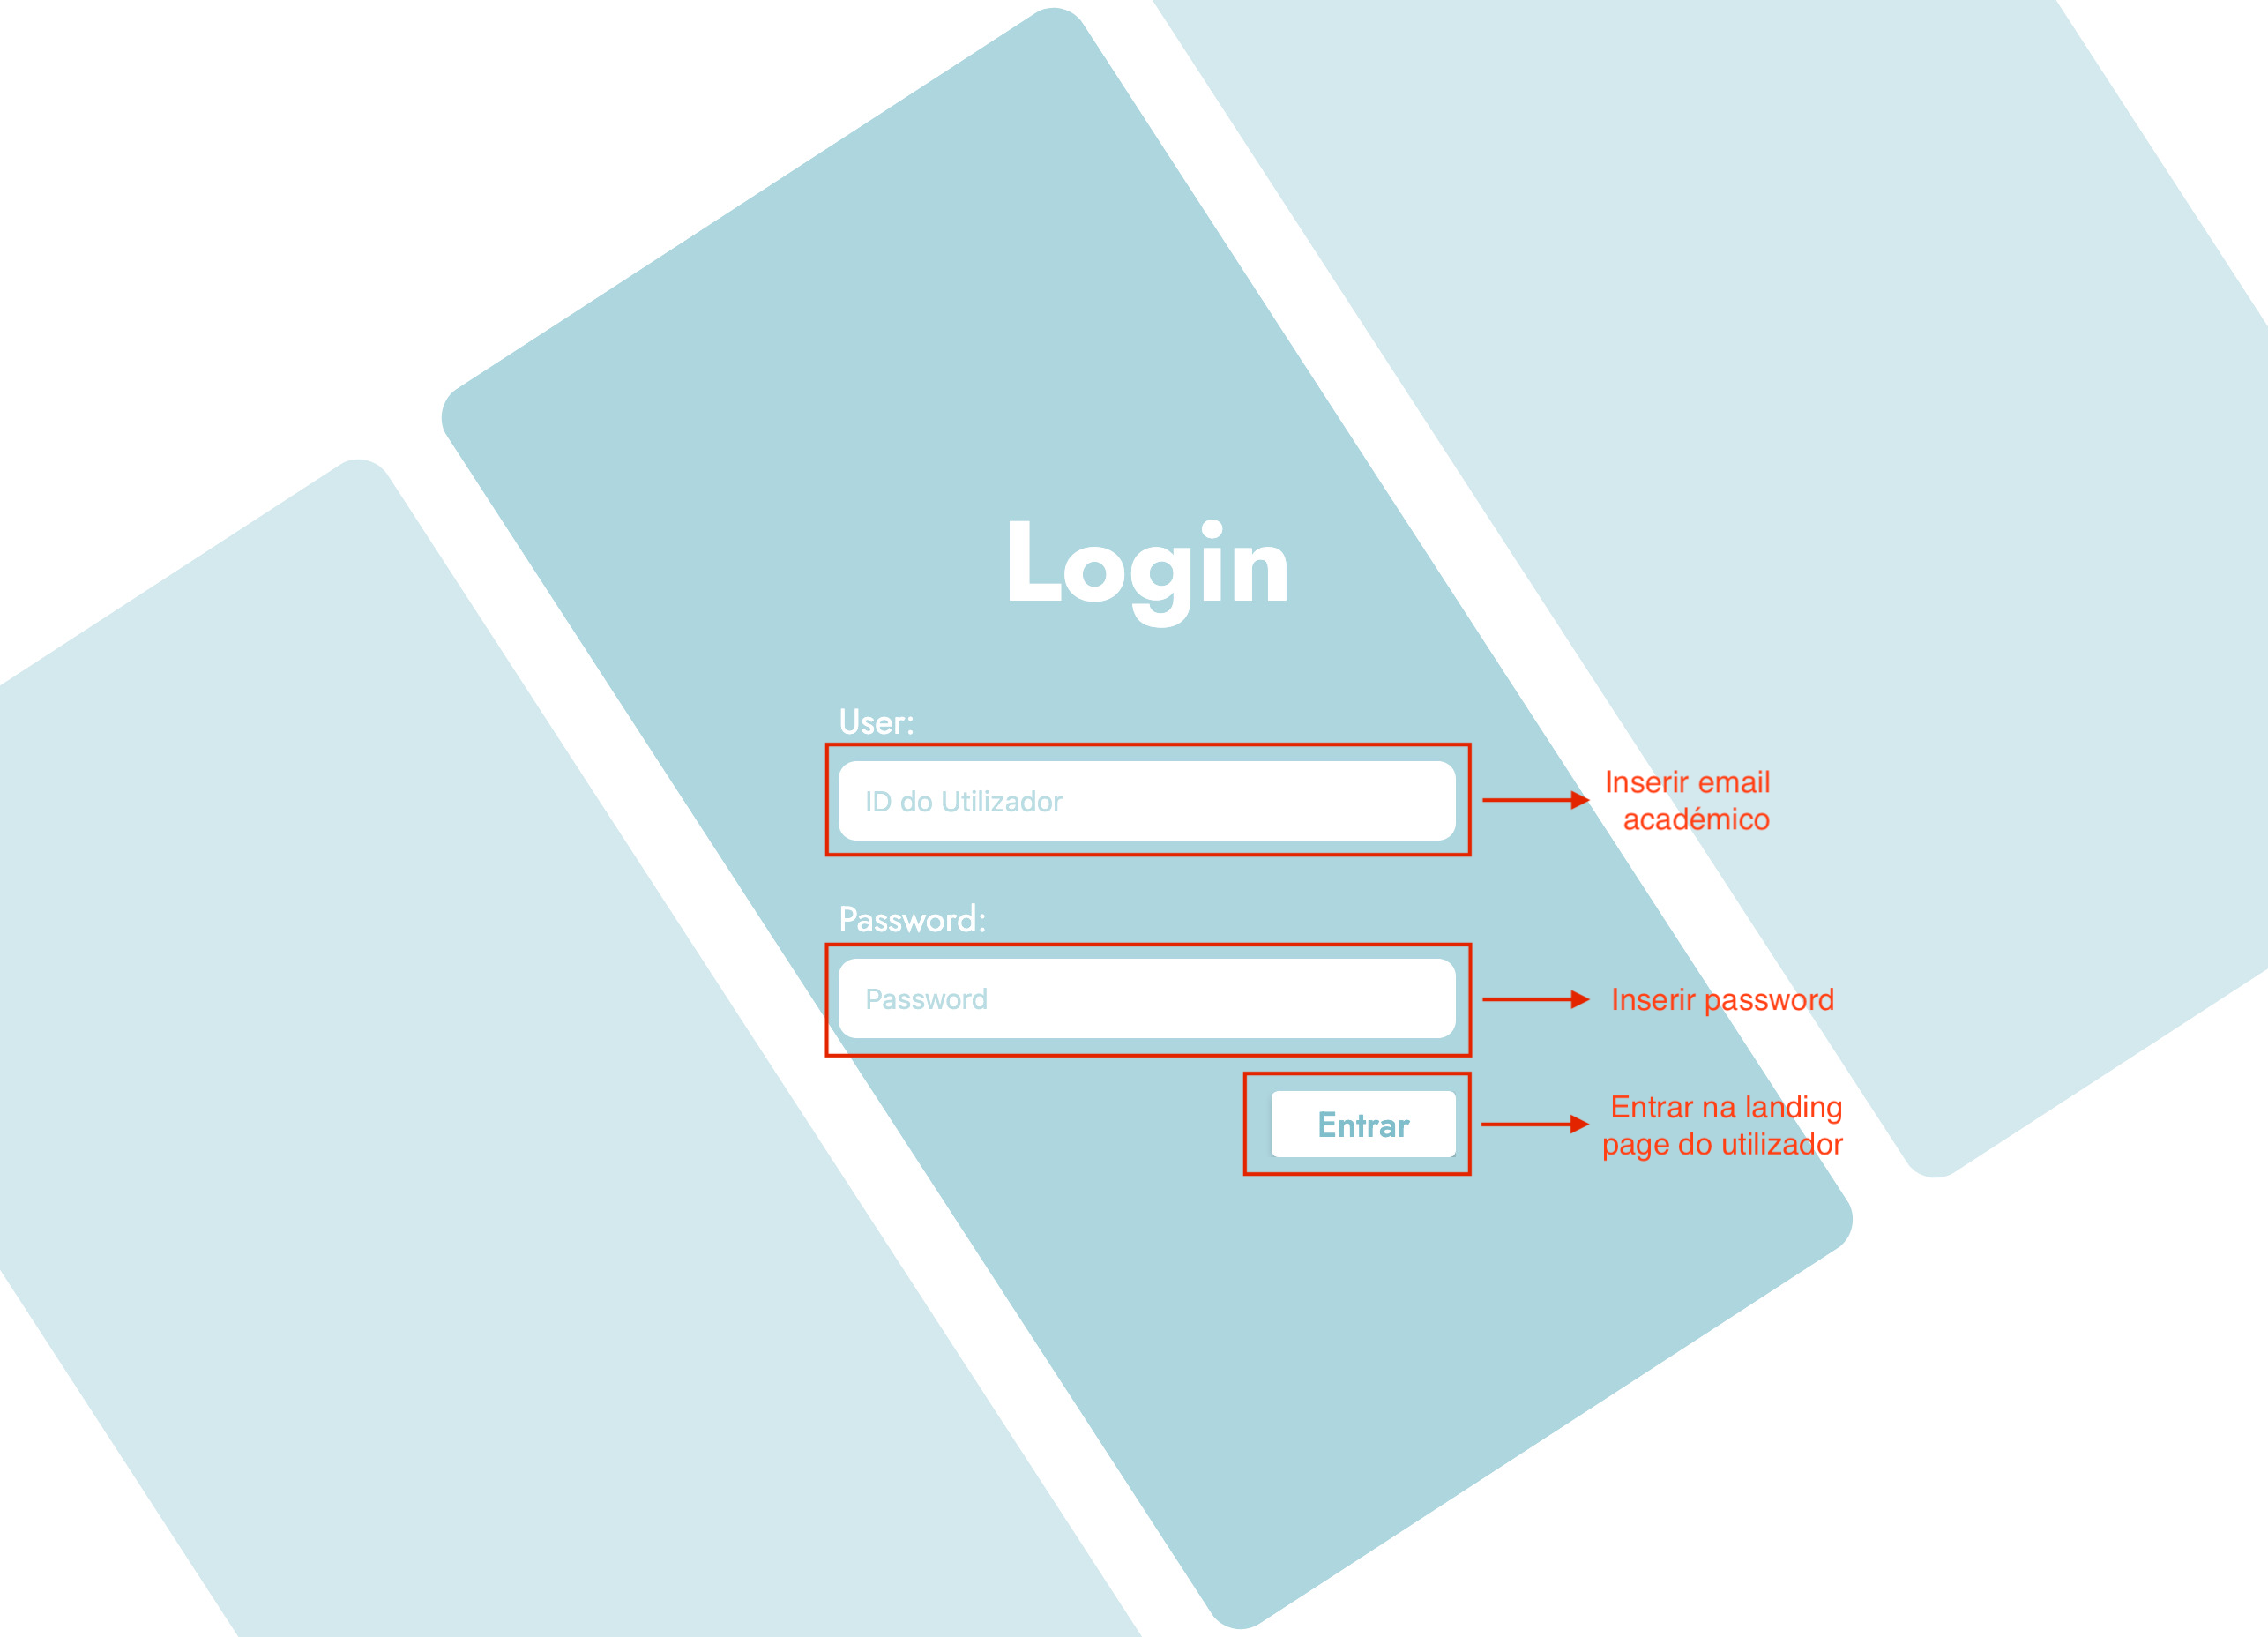
\includegraphics[width=0.75\linewidth]{manual/login-page.png}
    \caption{Página de Login}
    \label{fig:enter-label}
\end{figure}
Ao aceder à aplicação, o utilizador é encaminhado para a página de login. Como ilustrado na figura, deve introduzir as suas credenciais nos campos apropriados. Caso estejam corretas, será redirecionado para a sua página principal.
\begin{figure}[H]
    \centering
    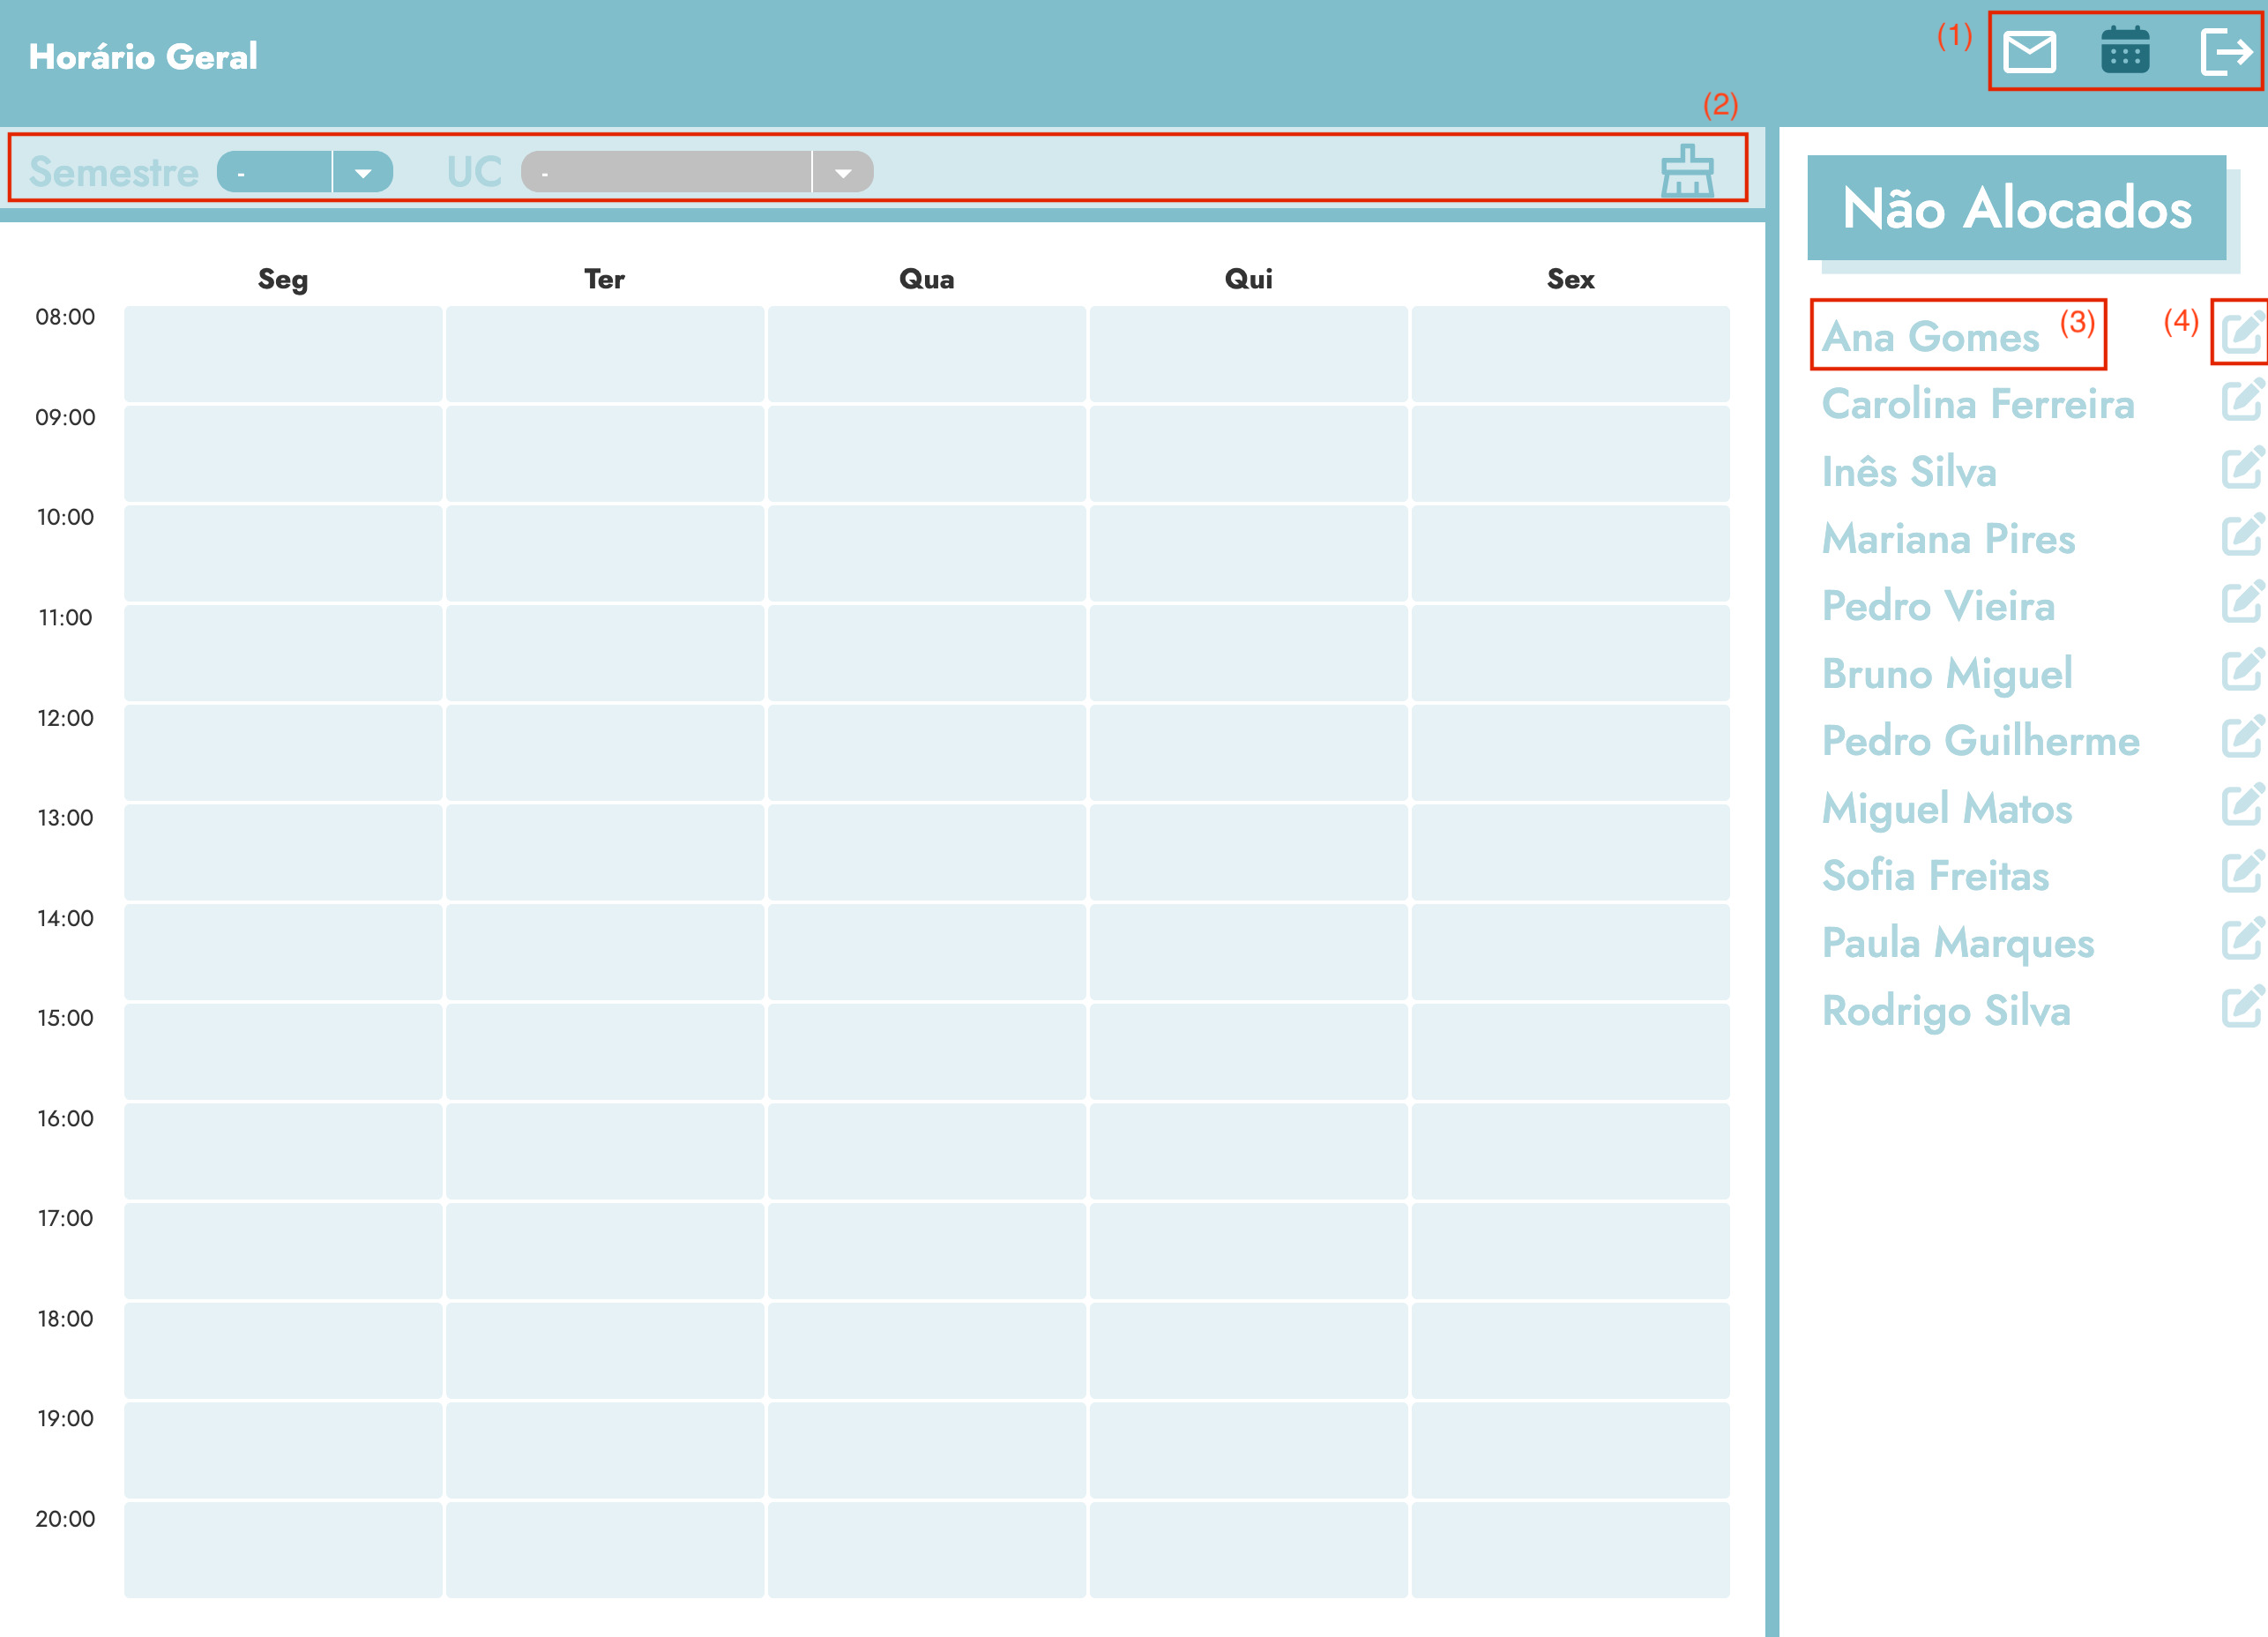
\includegraphics[width=0.49\linewidth]{manual/admin-page.png}
    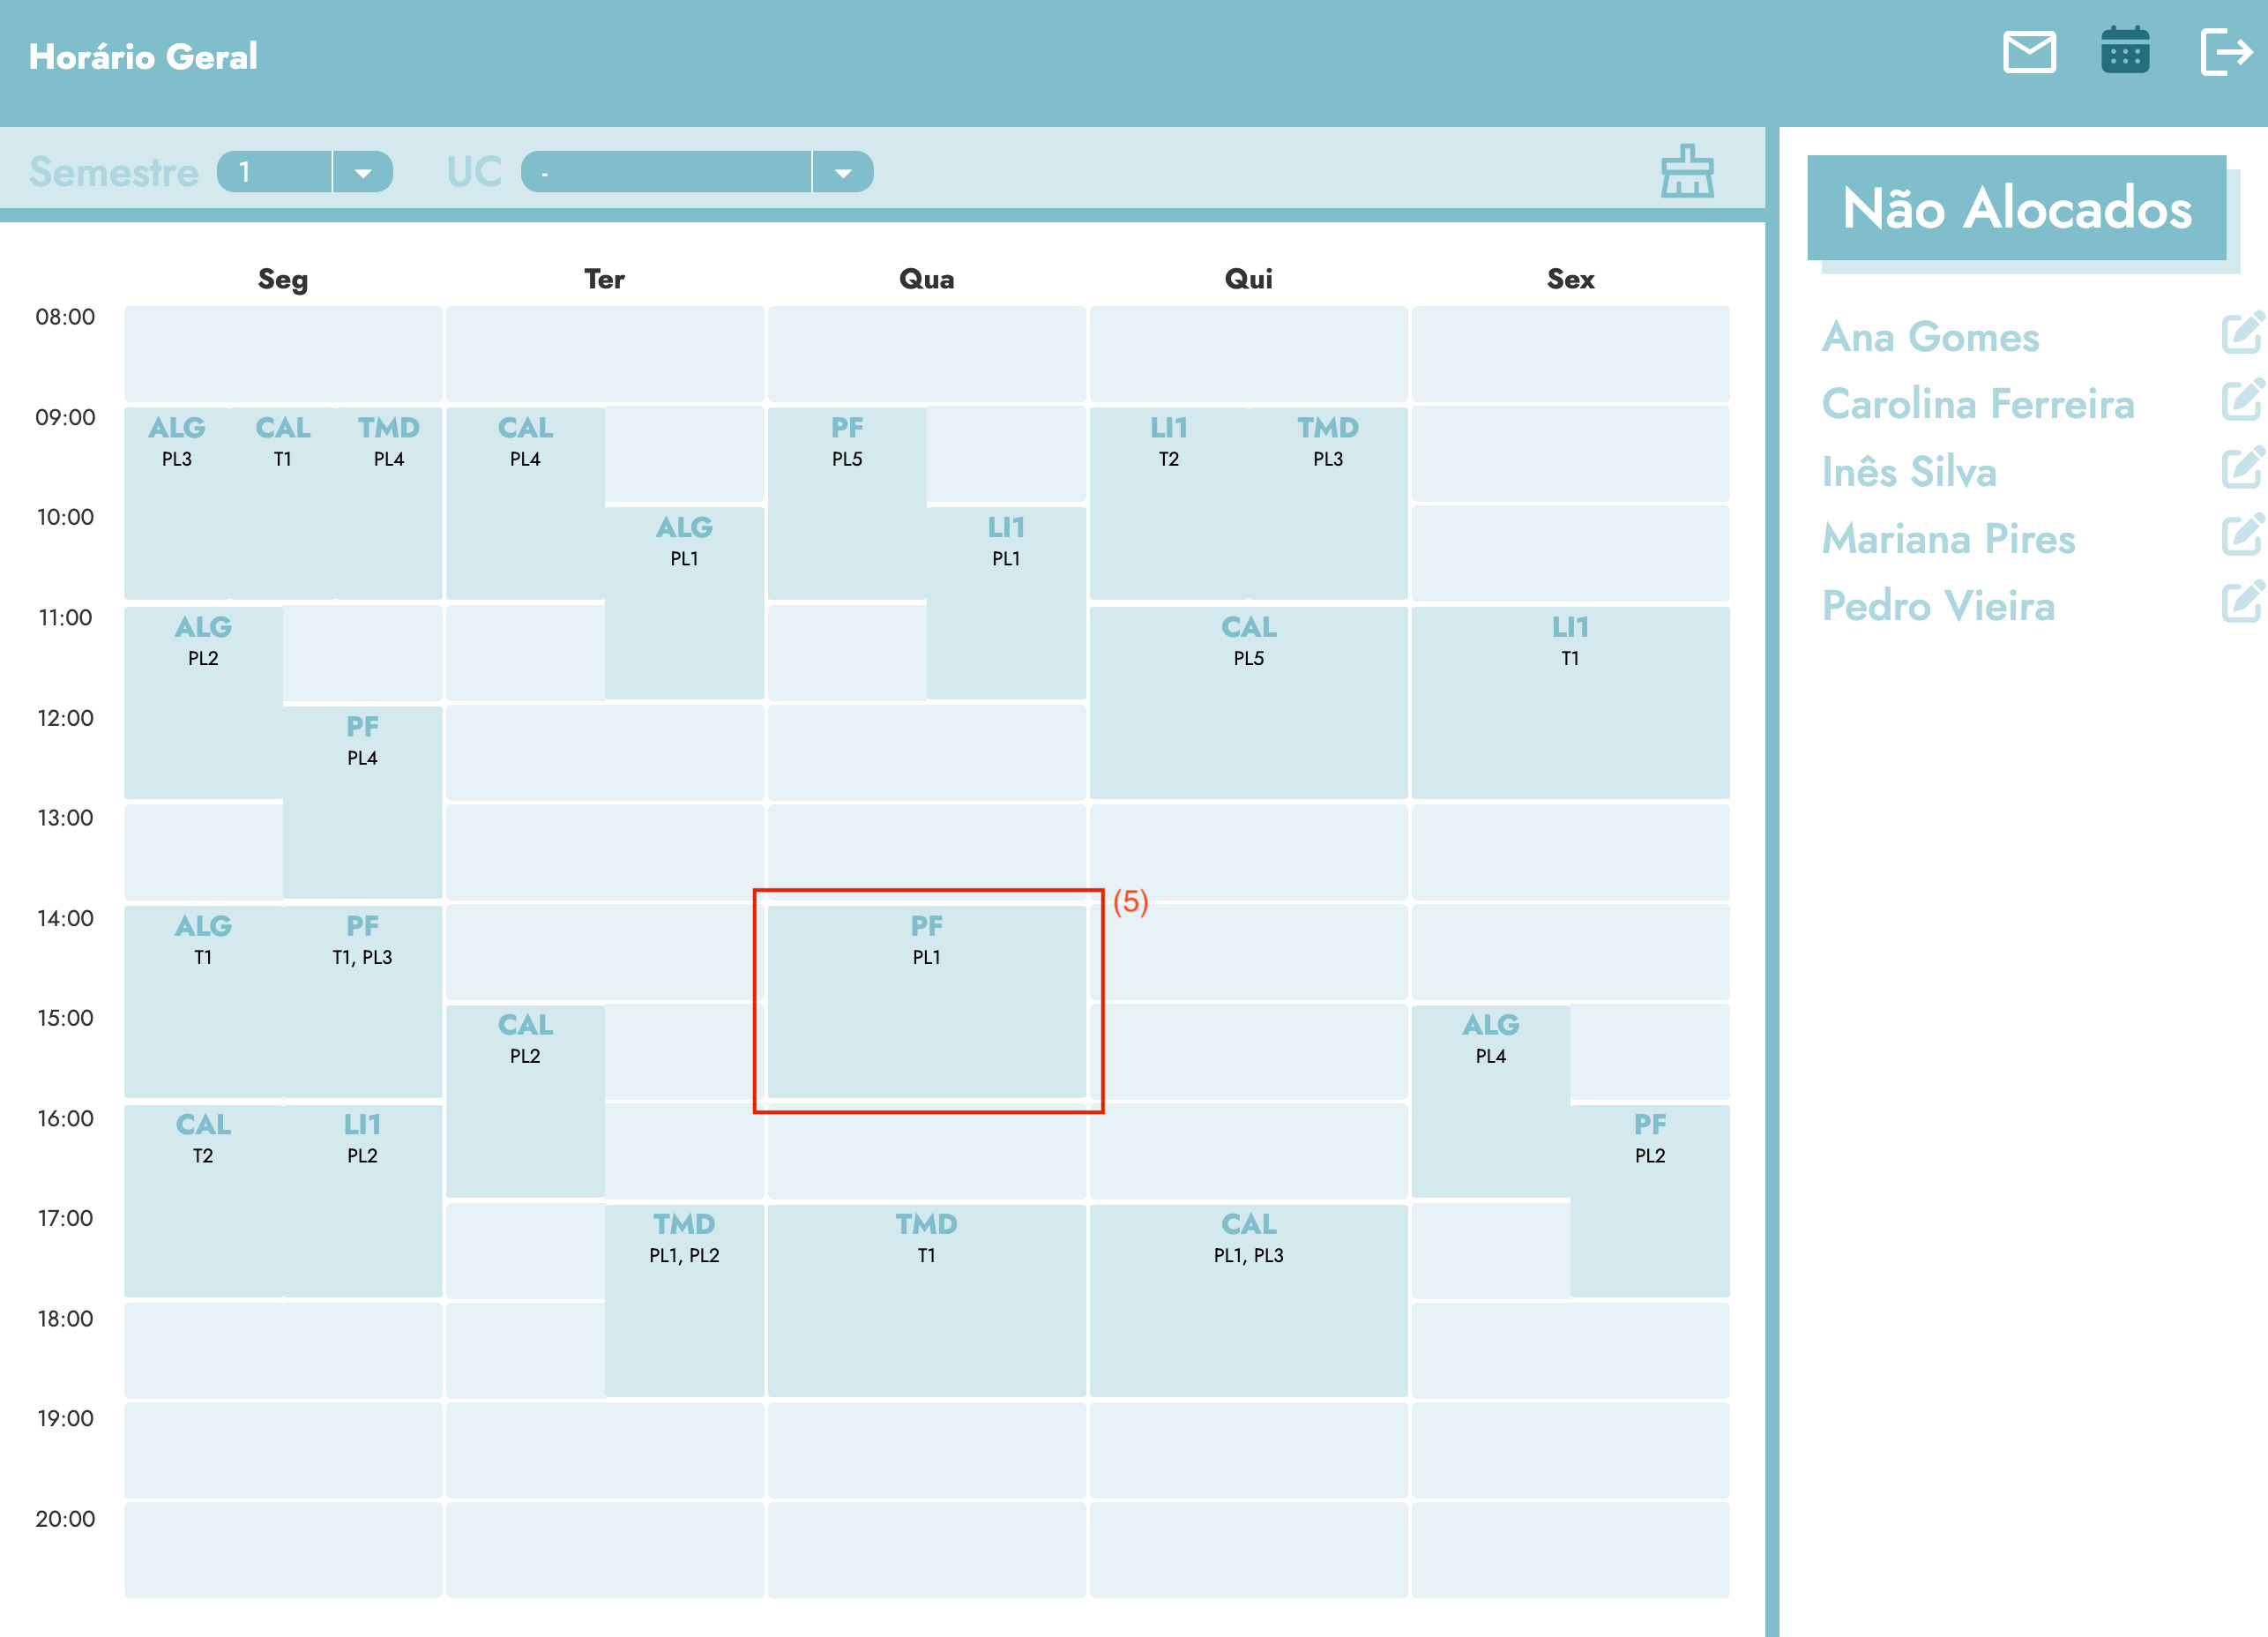
\includegraphics[width=0.49\linewidth]{manual/admin-with-calendar-page.png}
    \caption{Página do Diretor de Curso}
    \label{fig:enter-label}
\end{figure}
Se o utilizador for um diretor de curso, poderá realizar várias ações conforme o seu objetivo. A figura apresenta os diferentes componentes com os quais pode interagir:
\begin{enumerate}
    \item \textbf{Navegação} – O utilizador pode navegar para a página de mensagens clicando no ícone de envelope ou sair da aplicação através do botão de logout. O botão escurecido indica a rota atualmente ativa, estando desativado para prevenir a sua seleção.
    \item \textbf{Filtros de horário} – É possível selecionar entre os 6 semestres disponíveis (de 1 a 6) e, posteriormente, escolher uma Unidade Curricular (UC) correspondente. O botão à direita permite limpar os filtros aplicados. O filtro de UC apenas fica disponível após a seleção de um semestre.
    \item \textbf{Lista de Alunos} – O diretor pode clicar num aluno para abrir um popup com informações adicionais, descrito mais à frente neste relatório.
    \item \textbf{Editar Alocações} – Clicando no ícone correspondente, o utilizador é redirecionado para a página de edição de alocações do aluno selecionado.
    \item \textbf{Turnos no Horário} – Ao selecionar um turno no horário apresentado, são exibidos os detalhes desse turno específico.
\end{enumerate}
\begin{figure}[H]
    \centering
    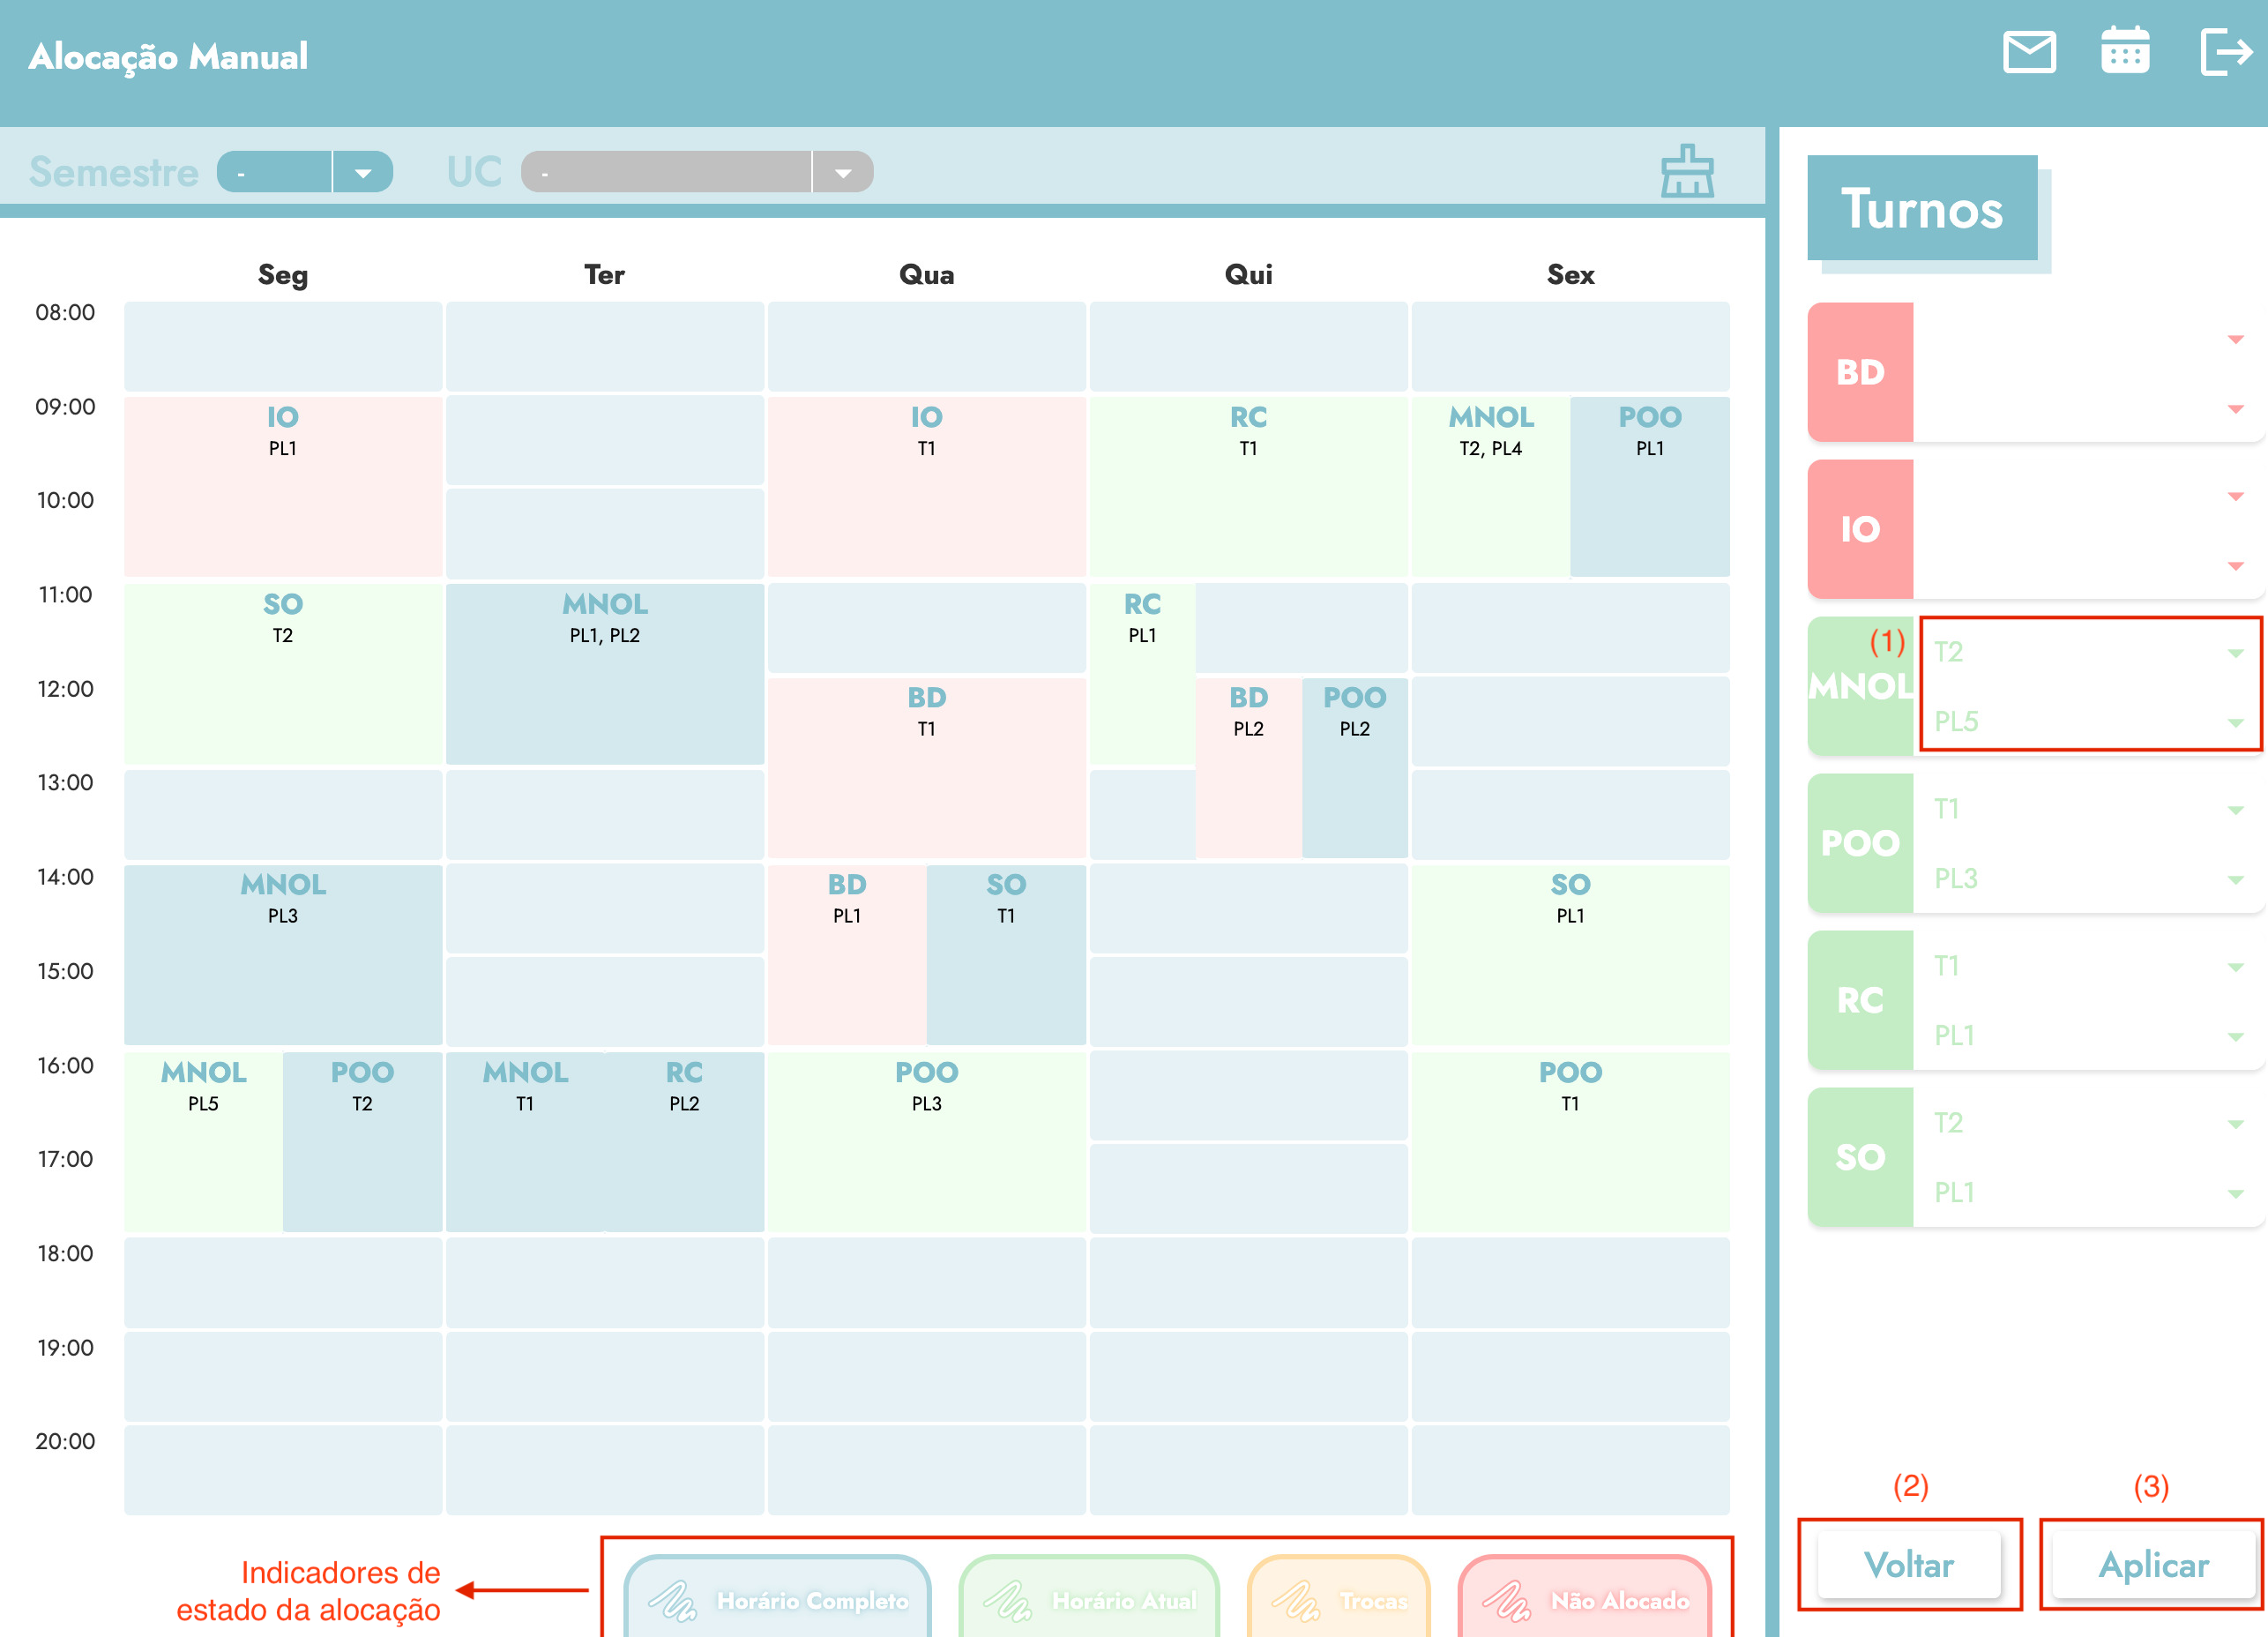
\includegraphics[width=0.75\linewidth]{manual/edit-page.png}
    \caption{Página de Edição de Alocações}
    \label{fig:enter-label}
\end{figure}
Após escolher um aluno, o diretor de curso é redirecionado para a página de edição das suas alocações. Esta página mantém os mesmos mecanismos de navegação e filtragem, com as seguintes funcionalidades adicionais:
\begin{enumerate}
    \item \textbf{Troca de Turnos} – O diretor pode clicar nos turnos atuais do aluno (o botão superior representa os turnos teóricos, o inferior os práticos), abrindo uma lista de turnos disponíveis para troca. A seleção de um turno reflete-se de forma reativa no estado do horário e dos turnos.
    \item \textbf{Cancelar Operação} – Em qualquer momento, o utilizador pode cancelar a operação e regressar à página anterior clicando no botão "Voltar".
    \item \textbf{Aplicar Alterações} – O botão "Aplicar" não confirma de imediato a alteração, mas abre um popup de confirmação para garantir a decisão do utilizador.
\end{enumerate}
\begin{figure}[H]
    \centering
    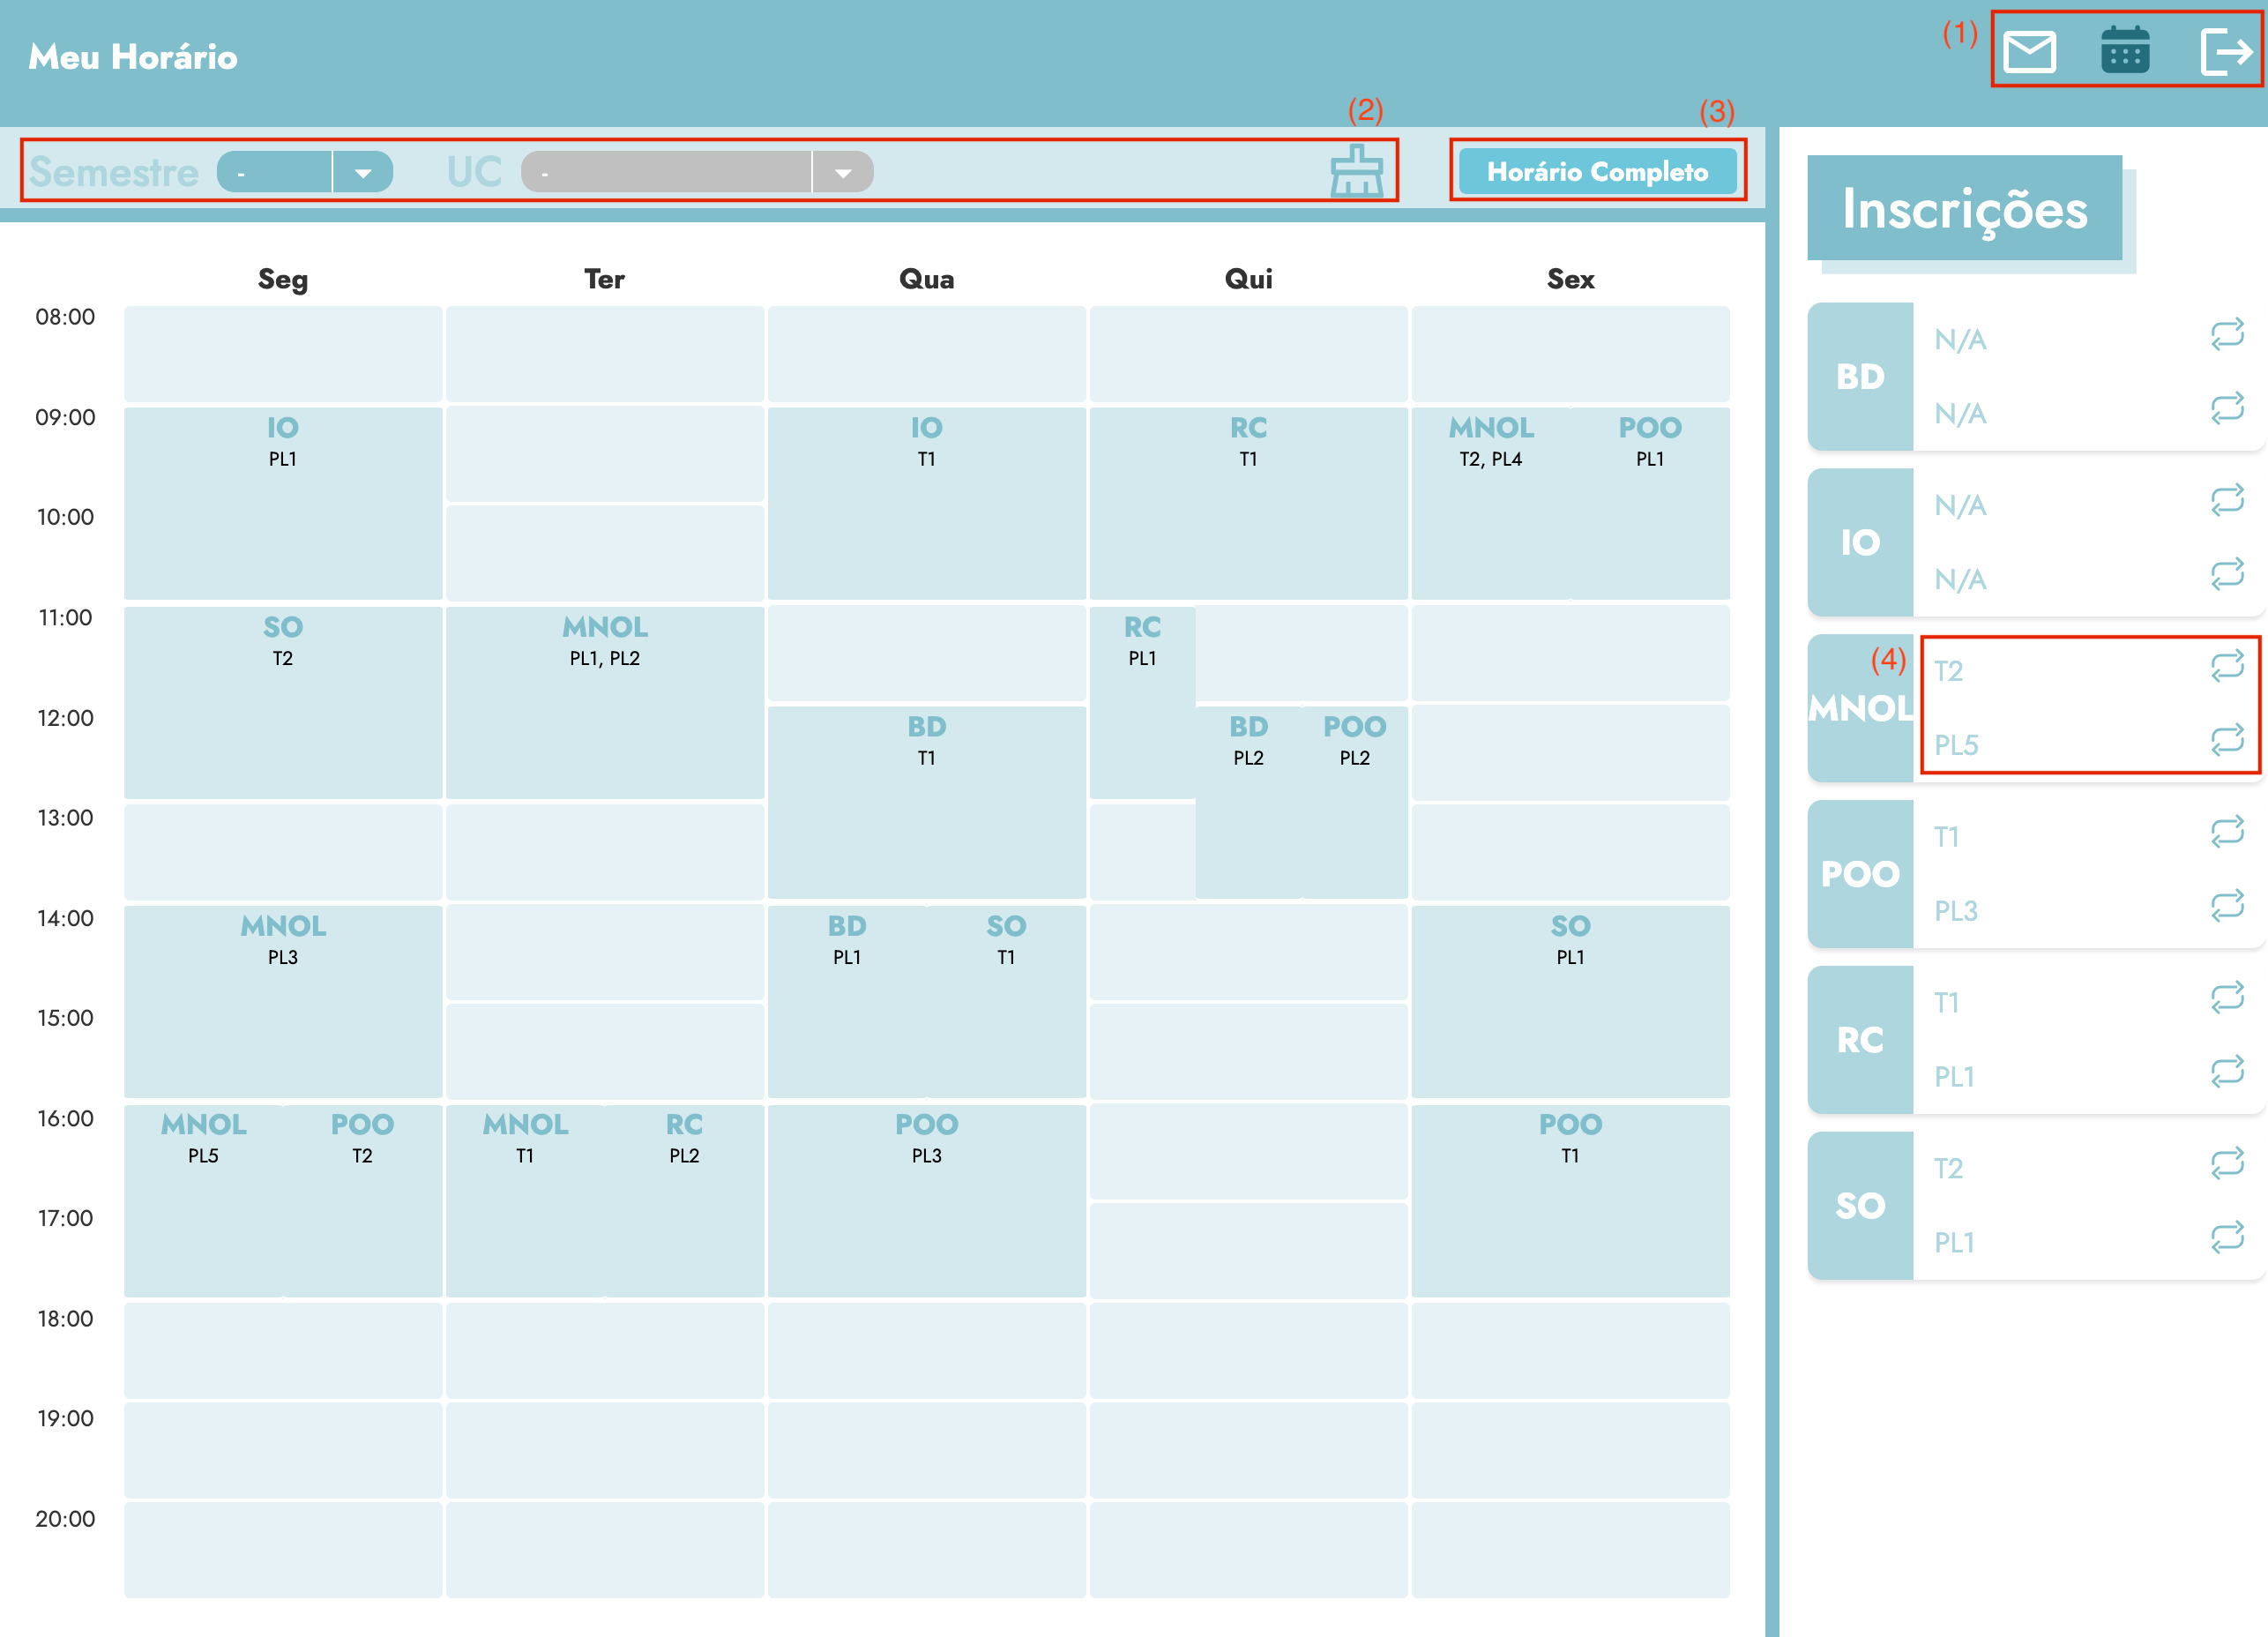
\includegraphics[width=0.75\linewidth]{manual/student-page.png}
    \caption{Página do Aluno}
    \label{fig:enter-label}
\end{figure}
Na página do aluno, muitas das funcionalidades são semelhantes às da página do diretor de curso, com algumas diferenças importantes. O aluno não necessita de aplicar filtros para visualizar o seu horário; este é carregado automaticamente com base nas UCs em que está inscrito.
\begin{enumerate}
    \item \textbf{Navegação} – Funciona da mesma forma, com redirecionamentos ajustados ao perfil do aluno autenticado.
    \item \textbf{Filtros} – Mantêm-se idênticos aos da página do diretor.
    \item \textbf{Alternância de Horário} – O botão permite alternar entre "Horário Completo" e "Horário Atual". O primeiro mostra todos os turnos das UCs em que o aluno está inscrito; o segundo mostra apenas os turnos nos quais está efetivamente alocado.
    \item \textbf{Pedido de Troca de Turno} – Ao clicar num turno no horário, é aberto um popup para o aluno requisitar a troca desse turno.
\end{enumerate}
\begin{figure}[H]
    \centering
    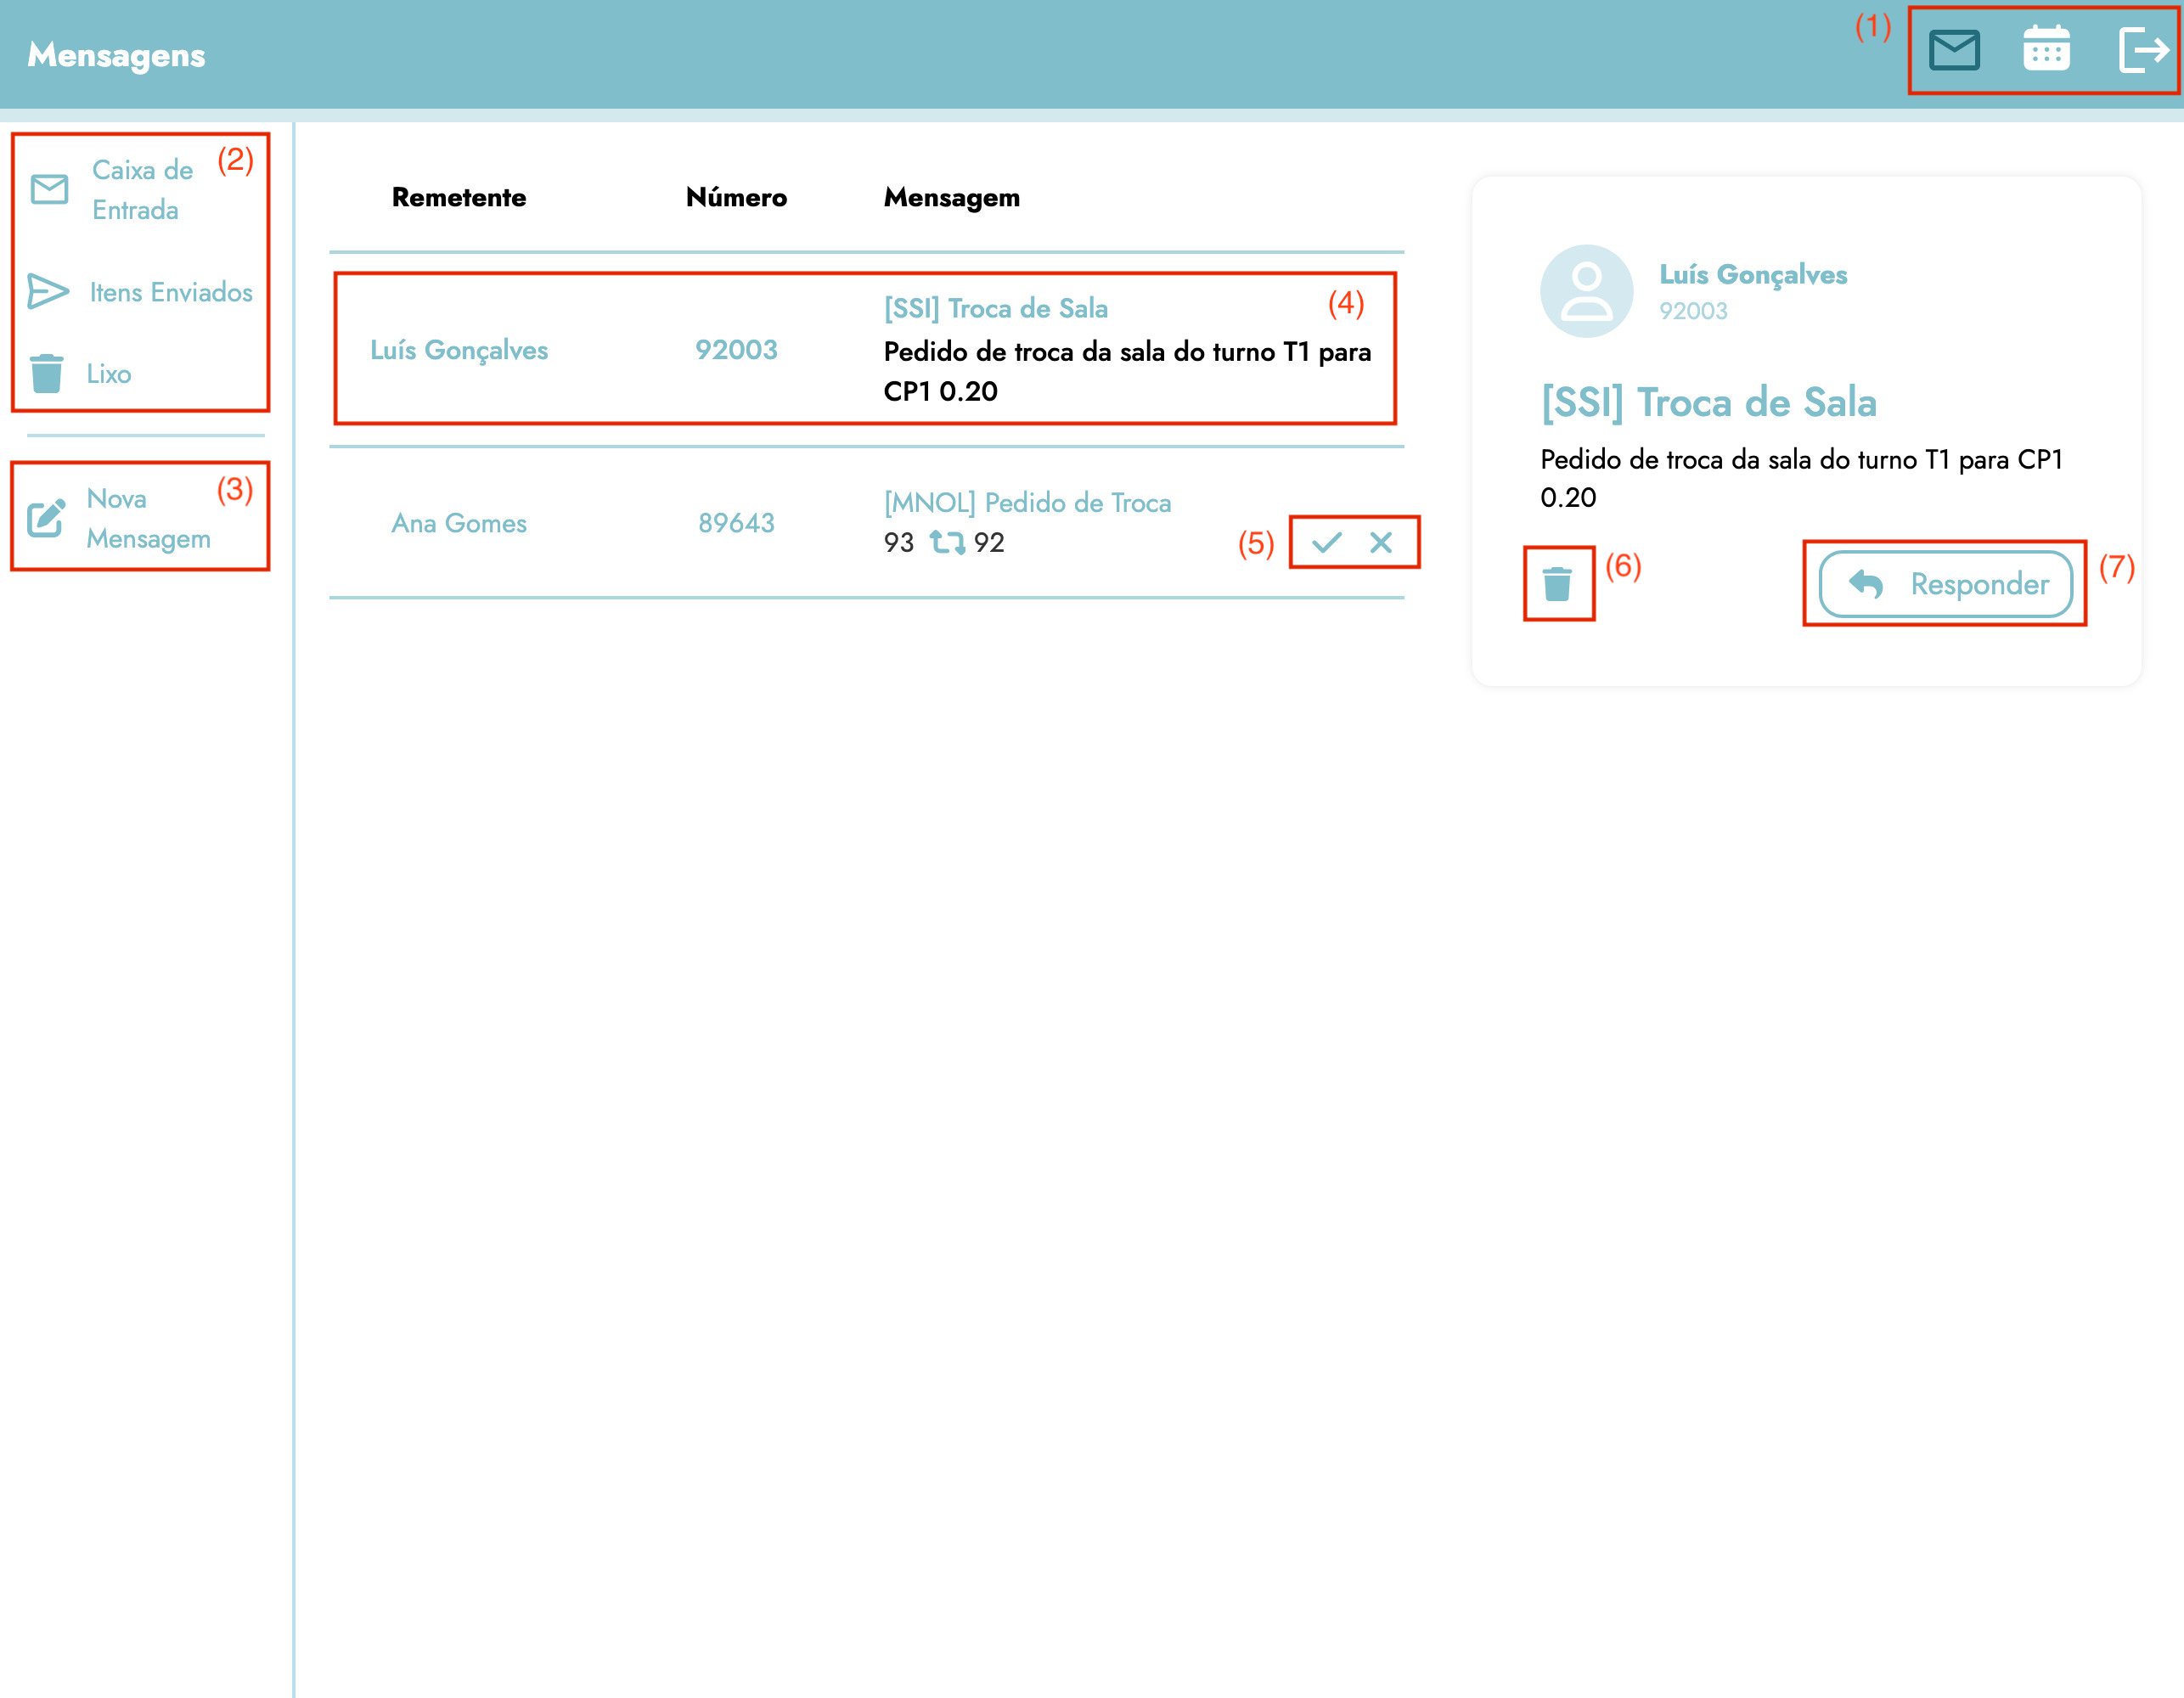
\includegraphics[width=0.49\linewidth]{manual/messages-page.png}
    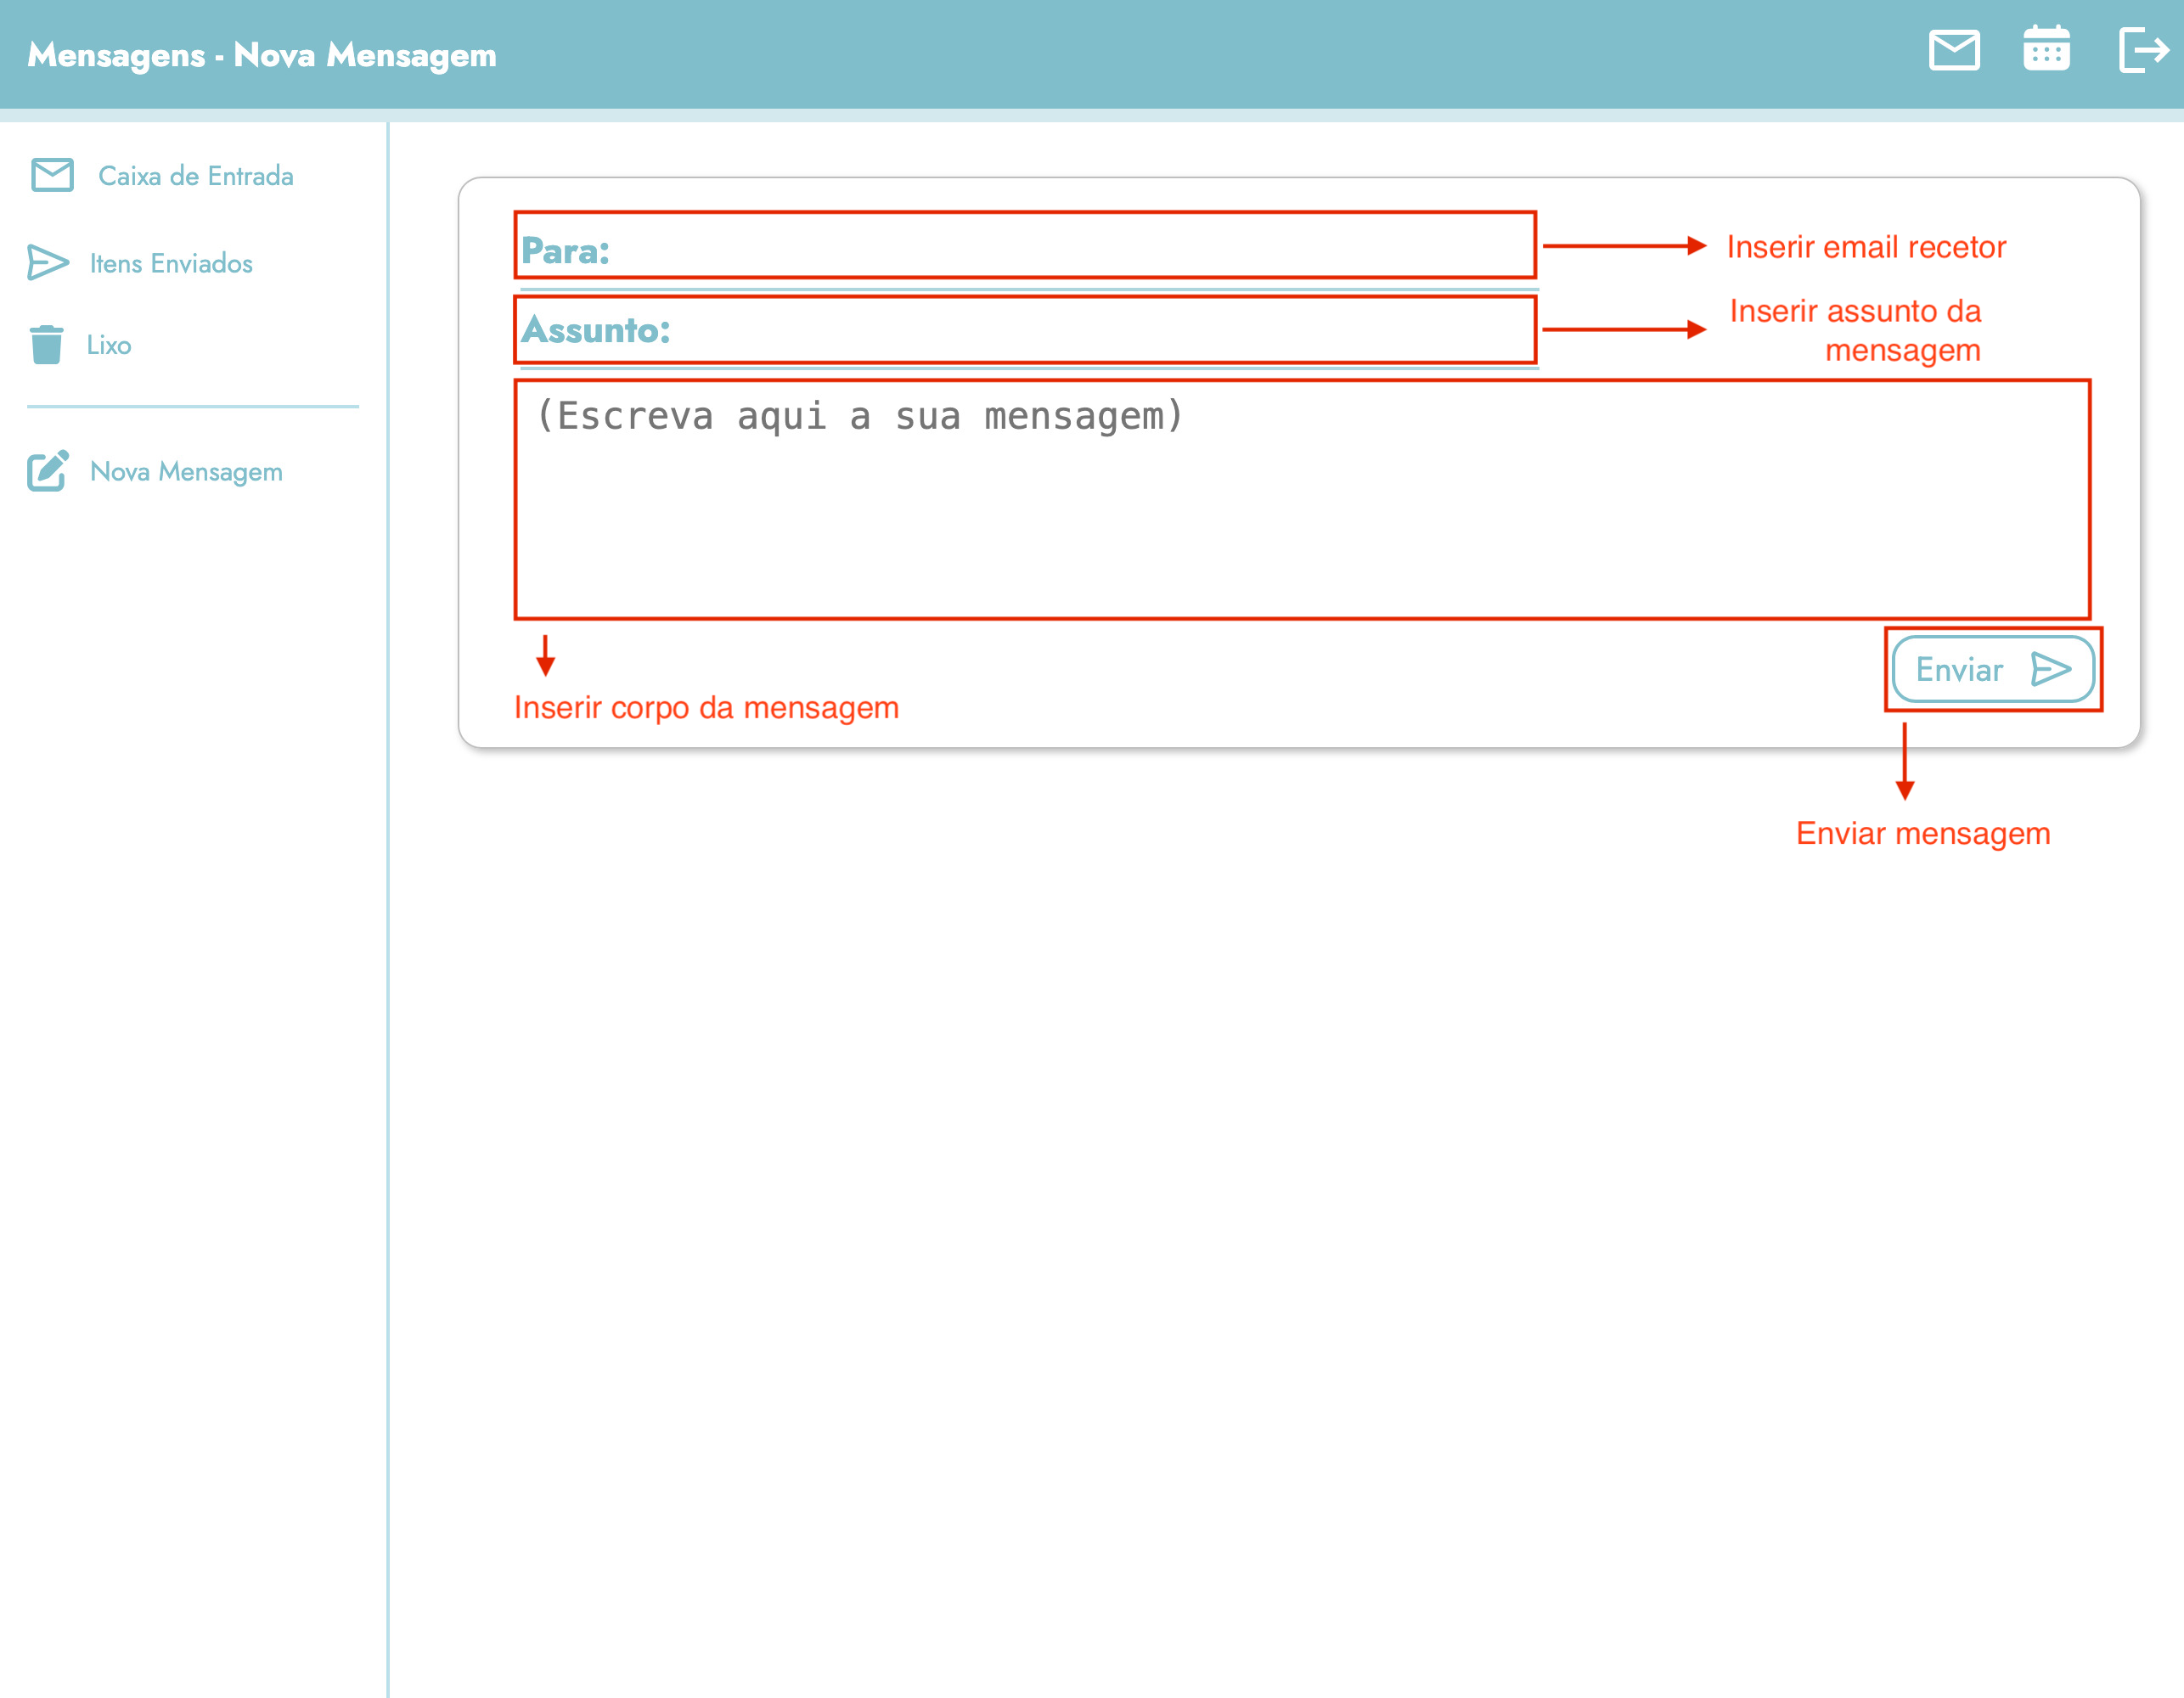
\includegraphics[width=0.49\linewidth]{manual/new-message-page.png}
    \caption{Páginas de Mensagens}
    \label{fig:enter-label}
\end{figure}
Tanto o diretor de curso como os alunos têm acesso à página de mensagens. Esta inclui as seguintes funcionalidades:
\begin{enumerate}
    \item \textbf{Navegação} – Mantém-se idêntica, com a secção de mensagens desativada (escurecida) por já estar ativa.
    \item \textbf{Caixas de Mensagens} – O utilizador pode navegar entre a caixa de entrada, mensagens enviadas e mensagens apagadas.
    \item \textbf{Nova Mensagem} – O botão "Nova mensagem" redireciona para a página de composição de mensagens.
    \item \textbf{Visualização Detalhada} – Ao clicar numa mensagem, esta é expandida para mostrar o conteúdo completo, bem como ações adicionais.
    \item \textbf{Troca Rápida} – Caso a mensagem seja de "troca rápida", o diretor de curso pode aceitá-la ou rejeitá-la diretamente nesta página.
    \item \textbf{Apagar a Mensagem} – O utilizador pode apagar a mensagem expandida, movendo-a para a caixa de mensagens apagadas.
    \item \textbf{Responder a Mensagem} – O utilizador pode optar por responder a uma mensagem, sendo redirecionado para a página de composição, com os campos "Para" e "Assunto" já preenchidos.
\end{enumerate}

\subsection{Descrição dos Popups}
\begin{figure}[H]
    \centering
    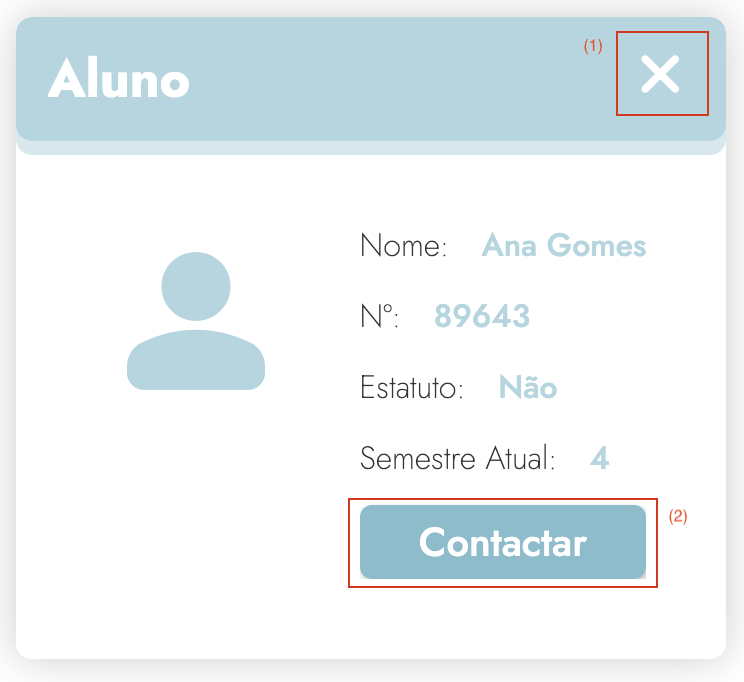
\includegraphics[width=0.3\linewidth]{manual/student-info-popup.png}
    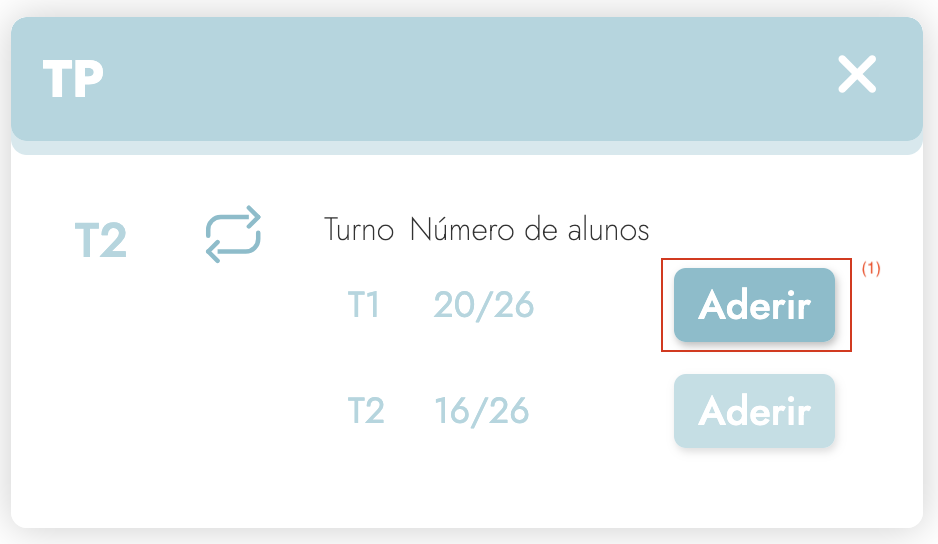
\includegraphics[width=0.3\linewidth]{manual/request-shift-change-popup.png}
    \label{fig:enter-label}
\end{figure}
Para os popups de \textbf{informações adicionais acerca do aluno} e \textbf{requisição de troca de turno}, o utilizador pode, respetivamente:
\begin{enumerate}
    \item \textbf{Fechar o Popup} - A qualquer momento, clicando no botão de fecho disponível, o utilizador pode fechar o popup. Esta funcionalidade está presente em todos os popups da aplicação, com efeito consistente.
    \item \textbf{Contactar} - Redireciona o diretor de curso para a página de composição de mensagens, com o campo “Para” já preenchido com o email do aluno em questão.
\end{enumerate}
\noindent\makebox[\linewidth]{\rule{0.2\textwidth}{0.2pt}}
\begin{enumerate}
    \item \textbf{Aderir} - Ação que envia automaticamente uma mensagem de “troca rápida” para o diretor de curso, formalizando o pedido de troca de turno.
\end{enumerate}
\begin{figure}[H]
    \centering
    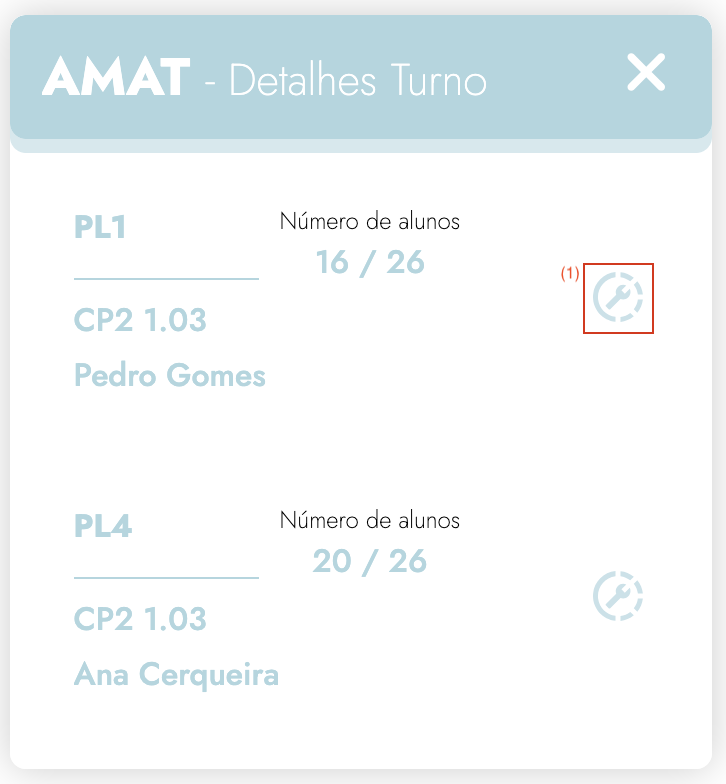
\includegraphics[width=0.3\linewidth]{manual/shit-details-popup.png}
    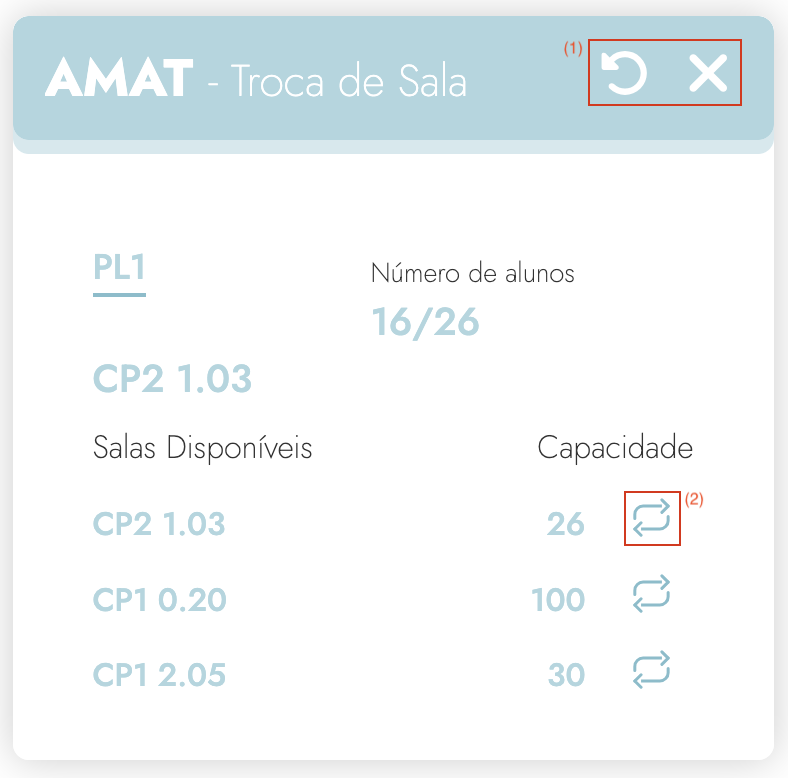
\includegraphics[width=0.3\linewidth]{manual/shift-change-room-popup.png}
    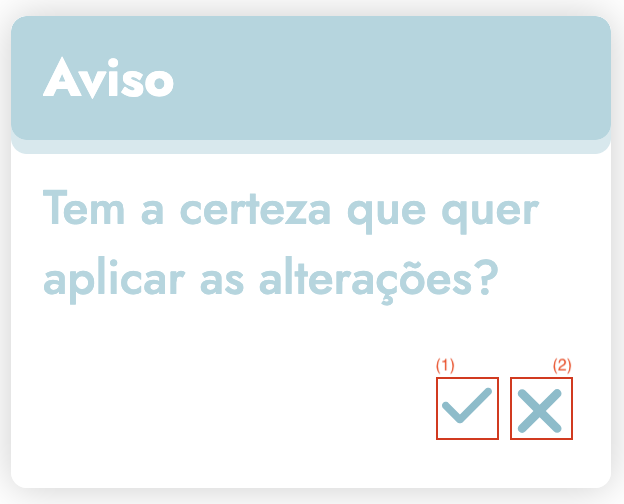
\includegraphics[width=0.3\linewidth]{manual/edit-confirmation-popup.png}
    \label{fig:enter-label}
\end{figure}
Para os popups de detalhes de turno, troca de sala e avisos, o utilizador pode, respetivamente:
\begin{enumerate}
    \item \textbf{Editar Sala} - Ao clicar no ícone de edição, o estado do popup avança para o próximo estado (troca de sala).
\end{enumerate}
\noindent\makebox[\linewidth]{\rule{0.2\textwidth}{0.2pt}}
\begin{enumerate}
    \item \textbf{Recuar} - O utilizador pode, além de poder fechar o popup a qualquer momento, recuar do estado atual.
    \item \textbf{Selecionar Sala} - seleciona a nova sala para o turno, o que abrirá um novo popup com um aviso de confirmação.
\end{enumerate}
\noindent\makebox[\linewidth]{\rule{0.2\textwidth}{0.2pt}}
\begin{enumerate}
    \item \textbf{Aceitar} - O utilizador aceita e reconhece o aviso.
    \item \textbf{Recusar} - O utilizador recusa aviso e cancela a operação.
\end{enumerate}

\newpage
\section{Reflexão sobre o Trabalho}

Durante o desenvolvimento da aplicação, o grupo deparou-se com vários desafios técnicos e organizacionais, mas também com aprendizagens relevantes e uma perceção bastante positiva relativamente à utilização da \textit{framework} Vue.

\subsection*{Principais Dificuldades}

A maior dificuldade enfrentada esteve relacionada com a implementação de um sistema de \textit{stores} modular que conseguisse gerir corretamente o estado da aplicação e garantir sincronizações consistentes com a base de dados. Foi necessário pensar cuidadosamente na separação de responsabilidades entre os diferentes \textit{stores} e na forma como estes interagem entre si.
Adicionalmente, surgiram complexidades quando as ações de um \textit{store} tinham implicações em outros — por exemplo, aprovar uma mensagem de troca de turno obriga à atualização do estado de várias entidades em simultâneo. Gerir esta coordenação e garantir que os dados se mantêm consistentes tanto no cliente como no servidor exigiu planeamento, testes frequentes e algumas refatorizações do código.

\subsection*{Pontos Positivos e Opiniões do Vue}

Apesar das dificuldades, a experiência de desenvolvimento com Vue.js foi altamente positiva. De forma geral, a biblioteca mostra-se bastante intuitiva e a curva de aprendizagem foi rápida com o apoio adicional à documentação oficial.\newline
A estrutura reativa do Vue, aliada à simplicidade da sintaxe, permitiu desenvolver uma interface dinâmica com menos código do que seria necessário noutras soluções.\newline
Além disso, a integração com ferramentas modernas como Vite, Pinia e Vue Router tornou o processo de desenvolvimento mais eficiente e modular. A funcionalidade de \textit{hot reload}, por exemplo, reduziu consideravelmente o tempo de testes e ajustes durante a fase de implementação.\newline

\end{document}